\documentclass[useAMS,usenatbib]{mn2e}
\usepackage[toc,page]{appendix}
\usepackage{natbib}
\usepackage{amssymb}
\usepackage{epsf}
\usepackage{pstricks}
\usepackage{color}
\usepackage{graphicx}
\usepackage{slashed}
\usepackage{relsize}
\usepackage{morefloats}
\usepackage{multirow}

%\usepackage {amsmath}
%\usepackage {amsxtra}
%\usepackage {amsbsy}
%\usepackage {amscd}
\usepackage {array}

%\usepackage {graphics}
%\usepackage {amsfonts}
%\usepackage {float}
%\usepackage {indentfirst}
%\usepackage{verbatim}

%\usepackage {a4wide}
%\usepackage {setspace}
%\usepackage{enumitem}
\usepackage{hyperref}
%\usepackage[all]{hypcap}
%\usepackage{caption}
\usepackage[justification=centering]{caption}

\newcommand{\nat}{Nature}
\newcommand{\mnras}{MNRAS}
\newcommand{\apj}{ApJ}
\newcommand{\apjl}{ApJL}
\newcommand{\apjs}{ApJS}
\newcommand{\aap}{A\&A}
\newcommand{\pasa}{PASA}
\newcommand{\apss}{ApSS}
\newcommand{\araa}{ARAA}
\newcommand{\aj}{Astron. J.}
\newcommand{\aaps}{A\&AS}
\newcommand{\aplett}{Astrophys. Lett.}
\newcommand{\cjaa}{ChJAA}

%\topmargin=-0.4in

%%%%%%%%%%%%%%%%%%%%%%%%%%%%%%%%%%%%%%%%%%%%%%%%%%%%%%%%%%%%%%%%%%%%%%
\bibliographystyle{mn2e}
\begin{document}

\title[A Study of the Multi-frequency Polarization Pulse Profiles of Millisecond Pulsars]{A Study of the Multi-frequency Polarization Pulse Profiles of Millisecond Pulsars}
\author[S. Dai et al.]{S. Dai$^{1,2}$, G. Hobbs$^1$, R. N. Manchester$^1$, M. Kerr$^1$, R. Shannon$^1$, W. van Straten$^3$,   
\newauthor A. Mata$^9$, M. Bailes$^3$, N. D. R. Bhat$^4$, S. Burke-Spolaor$^5$, W. A. Coles$^6$, S. Johnston$^1$, 
\newauthor M. J. Keith$^7$, Y. Levin$^8$, S. Os\l owski$^{10,11}$, D. Reardon$^{8,1}$, V. Ravi$^{12}$, J. M. Sarkissian$^{13}$, 
\newauthor C. Tiburzi$^{14,15,1}$, L. Toomey$^{1}$, H. G. Wang$^{16,1}$, J.-B. Wang$^{17}$, L. Wen$^{18}$, R. X. Xu$^{2,19}$, 
\newauthor W. M. Yan$^{17}$, X.-J. Zhu$^{18}$\\
$^1$CSIRO Astronomy and Space Science, Australia Telescope National Facility, Box 76 Epping NSW 1710, Australia\\
$^2$School of Physics and State Key Laboratory of Nuclear Physics and Technology, Peking University, Beijing 100871, China\\
$^3$Centre for Astrophysics and Supercomputing, Swinburne University of Technology, PO Box 218, Hawthorn, VIC 3122, Australia\\
$^4$International Centre for Radio Astronomy Research, Curtin University, Bentley, WA 6102, Australia\\
$^5$Department of Astronomy, California Institute of Technology, Pasadena, CA 91125, USA\\
$^6$Department of Electrical and Computer Engineering, University of California, San Diego, La Jolla, CA 92093, USA\\
$^7$Jodrell Bank Centre for Astrophysics, University of Manchester, M13 9PL, UK\\
$^8$School of Physics, Monash University, PO Box 27 Clayton, VIC 3800, Australia\\
$^9$Center for Advanced Radio Astronomy, University of Texas, Rio Grande Valley, Brownsville, TX 78520, USA\\
$^{10}$Max-Planck-Institut f\"{u}r Radioastronomie, Auf dem H\"{u}gel 69, D-53121 Bonn, Germany\\
$^{11}$Department of Physics, Universit\"{a}t Bielefeld Universit\"{a}tsstr. 25 D-33615 Bielefeld, Germany\\
$^{12}$School of Physics, University of Melbourne, Parkville, VIC 3010, Australia\\
$^{13}$CSIRO Astronomy and Space Science, Parkes Observatory, Box 276, Parkes NSW 2870, Australia\\
$^{14}$INAF–Osservatorio Astronomico di Cagliari, Via della Scienza, I-09047 Selargius (CA), Italy\\
$^{15}$Dipartimento di Fisica, Universit\`a di Cagliari, Cittadella Universitaria, I-09042 Monserrato (CA), Italy\\
$^{16}$School of Physics and Electronic Engineering, Guangzhou University, 510006 Guangzhou, China\\
$^{17}$Xinjiang Astronomical Observatory, Chinese Academy of Sciences, 150 Science 1-Street, Urumqi, Xinjiang 830011, China\\
$^{18}$Department of Physics, University of Western Australia, Crawley, WA 6009, Australia\\
$^{19}$Kavli Institute for Astronomy and Astrophysics, Peking University, Beijing 100871, China\\
}

\maketitle

\begin{abstract}

We present high signal-to-noise ratio, multi-frequency polarization profiles 
for $24$ millisecond pulsars that are being observed as part of the Parkes 
Pulsar Timing Array (PPTA) project. 
%
The pulsars are observed in three bands, centered close to $730$, $1400$
and $3100$ MHz, using a dual-band 10\,cm/50\,cm receiver and the 
central beam of the 20\,cm multibeam receiver. 
%
Observations spanning many years have been carefully calibrated and summed to 
produce high S/N profiles. This allows us to study the individual profile 
components and how they evolve with frequency. We also identify previously undetected 
profile features.   
%
For many pulsars we show that pulse components exist across almost the entire 
pulse profile. The pulse component widths and component separations follow a complex 
evolution with frequency; in some cases these parameters increase and in other cases 
they decrease with increasing frequency. 
%
The evolution with frequency of the polarisation properties of the profile is also 
non-trivial. We provide evidence that the pre- and post-cursors generally have higher 
fractional linear polarization than the main pulse.  
%
We have obtained the spectral index and rotation measure for each pulsar by 
fitting across all three observing bands. For the majority of pulsars these parameters 
follow our expectation with a single power-law fitting the spectra and the position angles 
following the frequency-squared law. However, clear deviations are seen for some 
pulsars.  
%
We also present phase-resolved measurements of the spectral index, fractional linear 
polarisation and rotation measure. All these properties are shown to vary systematically 
over the pulse profile.

\end{abstract}



\begin{keywords}
%
pulsars: general
%
\end{keywords}


\section{Introduction}

Millisecond pulsars (MSPs) are a special subgroup of radio pulsars. 
%
Compared with ``normal'' pulsars, they have much shorter spin periods 
and smaller spin-down rates, and therefore have larger characteristic 
ages and weaker implied dipole magnetic fields.
%
The short spin periods and highly stable average pulse shapes of MSPs 
make them powerful tools to investigate a large variety of astrophysical phenomena.
In particular, much recent work has been to search for a gravitational wave background using 
observations of a large sample of MSPs in a ``Pulsar Timing Array"~\citep[e.g.,][]{Foster90}.
%
The Parkes Pulsar Timing Array (PPTA) project (Manchester et al. 2013) 
regularly observes $24$ MSPs. 
%
The PPTA search for gravitational waves has been described in other papers 
including~\citet{Shannon13b},~\citet{Wang14} and~\citet{Zhu14}. 
%

We have not yet detected gravitational waves. In order to do so we will need 
to observe a larger set of pulsars, increase the span of the observations and/or 
to increase the timing precision achieved for each observation. 
%To detect gravitational waves, we could observe a larger set of pulsars 
%and increase the span of the observations, but also to increase the timing 
%precision of the PPTA data set.
%
%requires that the pulse arrival times are measured with 
%a precision and accuracy of $\sim100$ ns over decades. 
%
%This requires that the pulse profiles are measured with high signal-to-noise 
%ratio and are stable over long time spans.  
%
Determining whether it is possible to improve the timing precision and, if so, 
by how much relies on our understanding of the stability of pulse profiles~\citep[e.g.,][]{Shannon14} 
and also on the profile frequency evolution and polarization properties.
%
For our work we study the large number of well calibrated, high signal-to-noise 
ratio (S/N) multi-frequency polarization profiles that have been obtained as 
part of the PPTA project. 
%

An earlier analysis of the 20\,cm pulse profiles from the PPTA sample was published by
~\citet{Yan11}. This earlier work is extended in this paper as:
%
(1) we include an extra four pulsars that have recently been added to the PPTA sample;
(2) we use more modern pulsar backend instrumentation than was available to~\citet{Yan11};
(3) we use longer data sets enabling higher S/N ratio profiles; and
(4) we provide polarization pulse profiles in three independent bands 
(at 10, 20 and 50\,cm).
%- we compare different models for different pulsar rotation measures
%
We note that, even though we have mainly the same sample of pulsars as was described by \citet{Yan11}, 
our data sets are independent (i.e., no data is in common between this and the earlier 
publication).

It has been shown that, compared with normal pulsars, the pulse profiles of MSPs are 
much more complicated and cover a much larger fraction of the pulse period~\citep{Yan11}. 
%
However, the spectra of MSPs and normal pulsars are similar~\citep{Toscano98,Kramer98,Kramer99}.
%
Both MSPs and normal pulsars often have a high degree of linear polarization and orthogonal 
mode position angle (PA) jumps~\citep[see e.g.,][]{Thorsett90,Navarro97,Stairs99,Manchester04,Ord04}.
%
For MSPs the PAs often varies significantly with pulse phase and, in most cases, they do not fit 
the `rotating vector model'~\citep[RVM,][]{Radhakrishnan69}.

To explain the complex pulse profiles, multiple emission cones were proposed 
and discussed by several authors~\citep{Rankin93,Kramer94b,Gupta03}. An alternative 
model suggests that the emission beam of a pulsar is filled with randomly 
distributed emission patches~\citep{Lyne88,Manchester95_2,Han01}. 
%
Based on investiagtions of the radio and $gamma$-ray beaming properties of both normal 
pulsars and MSPs,~\citet{Manchester05b} and~\citet{Ravi10} proposed that the radio emission 
of young and MSPs originates in wide beams from regions high in the pulsar magnetosphere 
and that features in the radio profile represent caustics in the emission beam pattern.
%

To date, no simple model exists yet that can describe the observations.  
%
%This paper is the first in a series of papers that we hope will shed new light on 
%the MSP emission mechanism. This first paper is an observationally-based 
%publication.  
This paper is an observationally-based publication that we hope will shed new 
light on the MSP emission mechanism.  
%
We present the new profiles in the various observing bands and describe how they were 
created. We determine various observationally-derived properties of the profiles (such as 
spectral indices, polarization fractions, etc.) and study how such parameters vary 
between pulsars and with frequency. 
%
Using these high S/N profiles, we also carry out phase-resolved studies on 
the spectral index~\citep[e.g.,][]{Lyne88,Kramer94a,Manchester04,Chen07}, linear polarization 
fraction and rotation measures (RMs)~\citep[e.g.,][]{Noutsos09}.
%
The data described here will be used in a subsequent paper to study the stability 
of the pulse profiles as a function of time. This sample of pulsars has been chosen for 
high-precision pulsar timing experiments. In a further paper, we will apply 
new methods~\citep[e.g.,][]{Pennucci14,Liu14} to improve our timing precision using 
frequency-dependent pulse templates.  
%
Our data sets are publically available enabling anyone to compare the actual 
observations with their models of the pulse profiles.
%

Details of the observation, data processing and data access are given in 
Section $2$. 
%
In Section $3$, we present the multi-frequency polarization pulse profiles.
%
The pulse widths, flux densities and spectral indices, polarization parameters 
and rotational measures are presented in Section $4$ to $7$. 
%
A summary of our results and conclusions are given in Section $8$.


\section{Observations and Analysis}

\subsection{Observations}

We selected observations from the PPTA project of $24$ MSPs. 
%
The pulsars are observed regularly, with an approximate observing cadence of 
three weeks, in three bands centred close to $730$ MHz (50\,cm), $1400$ MHz (20\,cm) and $3100$ MHz (10\,cm), 
using a dual-band 10\,cm/50\,cm receiver and the central beam 
of the 20\,cm multibeam receiver. The observing 
bandwidth was $64$, $256$ and $1024$ MHz respectively for the 50\,cm, 20\,cm 
and 10\,cm bands. 
%
We used both digital polyphase filterbank spectrometers (PDFB4 at 10\,cm 
and PDFB3 at 20\,cm) and a coherent dedispersion machine (CASPSR at 50\,cm). 
%
In Table \ref{obs}, we summarize the observational parameters for the $24$ PPTA MSPs. 
%Other basic pulsar parameters can be obtained from the ATNF 
%Pulsar Catalogue~\citep{Manchester05}.
%
For each band, we give the number of frequency channels across 
the band, the number of bins across the pulse period, the total number 
of observations and the total integration time.
%
In Table \ref{psr}, we give the basic pulsar parameters from the ATNF Pulsar 
Catalogue~\citep{Manchester05}.
%
For each observing band, we also give the dispersion smearing and the pulse 
broadening time caused by scattering (in units of profile bins).
%
The dispersion smearing across each frequency channel is calculated according to, 
%
\begin{equation}
\Delta t_{\rm{DM}}\approx 8.30 \times 10^{6}\ \rm{DM}\ \Delta \nu\ \nu^{-3}\ \rm{ms},
\label{dm}
\end{equation}
%
where $\Delta \nu$ is the channel width in MHz, $\nu$ is the band centre frequency in MHz, 
and the DM is in units of $\rm{cm^{-3}\ pc}$.
%
The pulse broadening time caused by scattering is estimated according to
%
\begin{equation}
\tau_{\rm{d}} = \frac{1}{2\pi\nu_0},
\end{equation}
%
where $\nu_0$ is the scintillation bandwidth. We calculate the broadening time 
in the 20\,cm band using scintillation bandwidths measured by~\citet{Keith13}, and 
then scale it to the 10\,cm and 50\,cm bands according to $\tau_{\rm{d}}\propto\nu^{-4}$.
For MSPs not in the sample of~\citet{Keith13}, we estimate the pulse broadening time 
using the empirical fit from \citet{Bhat04}, 
%
\[
\log \tau_{\rm{d}} = -6.46+0.154\log\rm{DM}+1.07(\log\rm{DM})^2
%\log \tau_{\rm{d}} = -6.46+0.154\log\rm{DM}+1.07(\log\rm{DM})^2-(3.86\pm0.16)\log\nu,
\]
%
\begin{equation}
	\qquad\quad\ \ -(3.86\pm0.16)\log\left(\frac{\nu}{1000}\right)\ \rm{ms}.
\label{scatter}
\end{equation}
%
We note that in Table \ref{psr}, we only list $\tau_{\rm{d}}$ values that are 
$\ge 0.0001\ \rm{bin}$ and set others as zero.


\begin{table*}
\caption{Observational parameters for the $24$ PPTA MSPs.}
\label{obs}
\begin{center}
%\begin{tabular}{lcccccccccccc}
\begin{tabular}{p{1.5cm}p{0.9cm}<{\centering}p{0.9cm}<{\centering}p{0.9cm}<{\centering}p{0.9cm}<{\centering}p{0.9cm}<{\centering}p{0.9cm}<{\centering}p{0.9cm}<{\centering}p{0.9cm}<{\centering}p{0.9cm}<{\centering}p{0.9cm}<{\centering}p{0.9cm}<{\centering}p{0.9cm}<{\centering}}
\hline
PSR         &     \multicolumn{3}{c}{No. of channels}   &   \multicolumn{3}{c}{No. of phase bins}  &    \multicolumn{3}{c}{No. of observation epochs}   &    \multicolumn{3}{c}{Integration time}      \\
%PSR         &         & No. of chan. &          &         & No. of bins &          &         & No. of obs. &          &         & Integ. time &          \\
            &         &                 &          &         &             &          &         &             &          &         &   (h)            &       \\
            & 50\,cm &    20\,cm     & 10\,cm &  50\,cm &    20\,cm     & 10\,cm &  50\,cm &    20\,cm     & 10\,cm &  50\,cm &    20\,cm     & 10\,cm     \\
%        & 730 &    1400     & 3100  & 730 &  1400   & 3100 & 730 &  1400  & 3100 & 730 &  1400 & 3100\\
%        &     &    (MHz)    &       &     &  (MHz)  &      &     &  (MHz) &      &     &  (MHz)&     \\
\hline
J0437$-$4715&  256    &    1024         &   1024   &  1024   &  1024       &  2048    &  177    &  669        & 281      &  142.9  &    502.2         &  248.8   \\
J0613$-$0200&  256    &    1024         &   1024   &  1024   &  512        &  512     &  64     &  160        & 111      &  66.0   &    159.3         &  113.9   \\
J0711$-$6830&  256    &    1024         &   1024   &  1024   &  1024       &  1024    &  72     &  161        & 102      &  65.9   &    161.1         &  102.2   \\
J1017$-$7156&  256    &    2048         &   2048   &  1024   &  256        &  512     &  85     &  135        & 73       &  86.5   &    130.4         &  76.3    \\
J1022$+$1001&  256    &    1024         &   1024   &  1024   &  2048       &  2048    &  65     &  148        & 117      &  58.4   &    138.3         &  110.5    \\
						&         &                 &          &         &             &          &         &             &          &         &                  &           \\
J1024$-$0719&  256    &    1024         &   1024   &  1024   &  1024       &  1024    &  34     &  112        & 59       &  36.1   &    111.0         &  61.5     \\
J1045$-$4509&  256    &    2048         &   1024   &  1024   &  512        &  1024    &  63     &  137        & 103      &  42.7   &    138.9         &  104.5    \\ 
J1446$-$4701&  256    &    512          &   1024   &  1024   &  512        &  1024    &  19     &  50         & 9        &  15.2   &    39.4          &  8.8    \\ 
J1545$-$4550&  256    &    1024         &   1024   &  1024   &  512        &  1024    &  15     &  21         & 15       &  13.2   &    20.6          &  12.2   \\ 
J1600$-$3053&  256    &    1024         &   1024   &  1024   &  512        &  512     &  53     &  139        & 106      &  56.6   &    129.9         &  108.0   \\ 
						&         &                 &          &         &             &          &         &             &          &         &                  &          \\
J1603$-$7202&  256    &    2048         &   1024   &  1024   &  1024       &  1024    &  52     &  131        & 49       &  44.4   &    127.4         &  50.6    \\ 
J1643$-$1224&  256    &    2048         &   1024   &  1024   &  512        &  1024    &  53     &  116        & 93       &  53.7   &    117.0         &  93.4     \\ 
J1713$+$0747&  256    &    1024         &   1024   &  1024   &  1024       &  1024    &  66     &  155        & 110      &  67.8   &    132.0         &  107.9    \\ 
J1730$-$2304&  256    &    1024         &   1024   &  1024   &  1024       &  2048    &  57     &  104        & 62       &  51.0   &    105.8         &  62.2    \\ 
J1744$-$1134&  256    &    512          &   1024   &  1024   &  1024       &  1024    &  65     &  129        & 96       &  66.0   &    126.7         &  99.5    \\ 
						&         &                 &          &         &             &          &         &             &          &         &                  &          \\
J1824$-$2453A&  256    &    2048         &   1024   &  1024   &  256        &  512     &  33     &  88         & 54       &  33.0   &    82.9          &  53.6    \\ 
J1832$-$0836&  256    &    1024         &   1024   &  1024   &  512        &  1024    &  12     &  19         & 11       &  9.0    &    16.9          &  10.1    \\ 
J1857$+$0943&  256    &    1024         &   1024   &  1024   &  1024       &  1024    &  54     &  99         & 68       &  27.8   &    50.9          &  35.5   \\ 
J1909$-$3744&  256    &    1024         &   1024   &  1024   &  512        &  1024    &  95     &  218        & 138      &  91.3   &    191.1         &  129.4   \\ 
J1939$+$2134&  256    &    1024         &   1024   &  512    &  256        &  256     &  58     &  102        & 91       &  26.4   &    49.4          &  46.0    \\ 
						&         &                 &          &         &             &          &         &             &          &         &                  &     \\
J2124$-$3358&  256    &    1024         &   1024   &  1024   &  1024       &  1024    &  40     &  134        & 78       &  20.3   &    68.5          &  40.5    \\ 
J2129$-$5721&  256    &    1024         &   1024   &  1024   &  512        &  512     &  59     &  116        & 17       &  31.1   &    112.6         &  9.0     \\ 
J2145$-$0750&  256    &    1024         &   1024   &  1024   &  2048       &  2048    &  70     &  134        & 117      &  65.1   &    129.3         &  111.2   \\ 
J2241$-$5236&  256    &    1024         &   1024   &  1024   &  512        &  1024    &  75     &  188        & 93       &  69.8   &    152.3         &  92.9   \\ 
\hline
\end{tabular}
\end{center}
\end{table*}

\begin{table*}
\caption{Pulsar parameters for the $24$ PPTA MSPs.}
\label{psr}
\begin{center}
\begin{tabular}{lcccccccc}
\hline
PSR         &   P     &       DM               &     \multicolumn{3}{c}{DM smear}   &   \multicolumn{3}{c}{$\tau_{\rm{d}}$}       \\
            &  (ms)   &  ($\rm{cm^{-3}\ pc}$)  &     \multicolumn{3}{c}{(bin)}      &   \multicolumn{3}{c}{(bins)}                \\
			      &         &                        &  50\,cm  & 20\,cm  & 10\,cm        & 50\,cm  &     20\,cm      & 10\,cm          \\
\hline
J0437$-$4715&  5.757  &  2.64             & 7.9      & 0.4       & 0.3       &    0.0004  &  0.0000  &  0.0000  \\ 
J0613$-$0200&  3.062  &  38.78            & 218.0    & 5.2       & 1.8       &    0.4058  &  0.0162  &  0.0006  \\ 
J0711$-$6830&  5.491  &  18.41            & 57.7     & 2.8       & 1.0       &    0.0103  &  0.0008  &  0.0000  \\ 
J1017$-$7156&  2.339  &  94.22            & 693.4    & 4.2       & 2.9       &    15.4014  &  0.3364  &  0.0287  \\ 
J1022$+$1001&  16.453 &  10.25            & 10.7     & 1.0       & 0.4       &    0.0019  &  0.0003  &  0.0000  \\ 
            &         &                   &          &           &           &            &          &          \\
J1024$-$0719&  5.162  &  6.49             & 21.6     & 1.0       & 0.4       &    0.0015  &  0.0001  &  0.0000  \\ 
J1045$-$4509&  7.474  &  58.17            & 133.9    & 1.6       & 2.2       &    2.9005  &  0.1160  &  0.0088  \\ 
J1446$-$4701&  2.195  &  55.83            & 437.8    & 21.1      & 7.3       &    1.8849  &  0.0823  &  0.0070  \\ 
J1545$-$4550&  3.575  &  68.39            & 329.2    & 7.9       & 5.5       &    2.5985  &  0.1135  &  0.0097  \\ 
J1600$-$3053&  3.598  &  52.33            & 250.3    & 6.0       & 2.1       &    6.2935  &  0.2516  &  0.0096  \\ 
            &         &                   &          &           &           &            &          &          \\
J1603$-$7202&  14.842 &  38.05            & 44.1     & 1.1       & 0.7       &    0.0275  &  0.0022  &  0.0001  \\ 
J1643$-$1224&  4.622  &  62.41            & 232.4    & 2.8       & 3.9       &    20.0424  &  0.8014  &  0.0610  \\ 
J1713$+$0747&  4.570  &  15.99            & 60.2     & 2.9       & 1.0       &    0.0186  &  0.0015  &  0.0001  \\ 
J1730$-$2304&  8.123  &  9.62             & 20.4     & 1.0       & 0.7       &    0.0202  &  0.0016  &  0.0001  \\ 
J1744$-$1134&  4.075  &  3.14             & 13.3     & 1.3       & 0.2       &    0.0083  &  0.0007  &  0.0000  \\ 
            &         &                   &          &           &           &            &          &          \\
J1824$-$2453A&  3.054  &  120.50           & 675.5    & 4.1       & 5.6       &    26.6882  &  0.5335  &  0.0406  \\ 
J1832$-$0836&  2.719  &  28.18            & 178.3    & 4.3       & 3.0       &    0.1321  &  0.0058  &  0.0005  \\ 
J1857$+$0943&  5.362  &  13.30            & 42.7     & 2.1       & 0.7       &    0.0691  &  0.0055  &  0.0002  \\ 
J1909$-$3744&  2.947  &  10.39            & 60.7     & 1.5       & 1.0       &    0.0187  &  0.0007  &  0.0001  \\ 
J1939$+$2134&  1.558  &  71.04            & 392.3    & 9.4       & 3.3       &    0.5451  &  0.0218  &  0.0008  \\ 
            &         &                   &          &           &           &            &          &          \\
J2124$-$3358&  4.931  &  4.60             & 16.0     & 0.8       & 0.3       &    0.0004  &  0.0000  &  0.0000  \\ 
J2129$-$5721&  3.726  &  31.85            & 147.1    & 3.5       & 1.2       &    0.0320  &  0.0013  &  0.0000  \\ 
J2145$-$0750&  16.052 &  9.00             & 9.7      & 0.9       & 0.3       &    0.0007  &  0.0001  &  0.0000  \\ 
J2241$-$5236&  2.187  &  11.41            & 89.8     & 2.1       & 1.5       &    0.0126  &  0.0006  &  0.0000  \\ 
%
\hline
\end{tabular}
\end{center}
\end{table*}

To calibrate the gain and phase of the receiver system, a linearly polarized 
broad-band and pulsed calibration signal is injected into the two orthogonal 
channels through a calibration probe at $45^{\circ}$ to the 
signal probes. The pulsed calibration signal was recorded for $2$ min prior to 
each pulsar observation.
%
Signal amplitudes were placed on a flux density scale using observations of 
Hydra A, assuming a flux density of 43.1\,Jy at 1400\,MHz and a spectral 
index of $\sim0.91$ over the PPTA frequency range.
%
All data were recorded using the PSRFITS data format~\citep{Hotan04} with 
$1$-min subintegrations and the full spectral resolution
%
\citep[for futher details see][and references therein]{Manchester13}. 
%(for futher details see~\citet{Manchester13}, and references therein). 
%

%Most of the pulsars in the sample show large flux variability at the PPTA 
%observing frequencies due to diffractive and refractive scintillation. 
%We find that for some of the pulsars in the PPTA sample show measured intensities 
%$> 20$ times of the mean; for these observations, Parkes observations can have S/N 
%in excess of larger aperture telescopes such as the Green Bank Telescope and 
%represent average observation with the MeerKAT telescope.
%


\subsection{Analysis}

The data were processed using the PSRCHIVE software package~\citep{Hotan04}. 
We removed 5 per cent of the bandpass at each edge and excised data 
affected by narrow band and impulsive radio-frequency interference for each 
sub-integration.
%
The polarization was then calibrated by correcting for differential gain and 
phase between the receptors using the associated calibration files.
%
For 20\,cm observations with the Multibeam receiver, we corrected for 
cross coupling between the feeds through a model derived from observations of 
PSR J0437$-$4715 that covered a wide range of parallactic angles~\citep{VanStraten04}.
%

The Stokes parameters are in accordance with the astronomical conventions described 
by~\citet{vanStraten10}. Stokes $V$ is defined as $I_{\rm{LH}}-I_{\rm{RH}}$, 
using the IEEE definition for sense of circular polarization. 
%
The linear polarization $L$ was calculated as $L=(Q^2+U^2)^{1/2}$, and the 
noise bias in $L$ was corrected according to~\citet{Lorimer05}, and the similar 
bias in $|V|$ was corrected as described in~\citet{Yan11}.
%
The position angles (PAs) of the linear polarization refer to the band central 
frequency and were calculated as $\psi=0.5\tan^{-1}(U/Q)$. They are absolute and 
measured from celestial north towards east, i.e. counterclockwise on the sky.
%
Errors on the PA values were estimated according to~\citet{Everett01}.
%
The baseline region was determined with the mean pulse profile using a default 
baseline duty cycle of 0.2 (for pulsars that different duty cycles were used, 
we give the value in their specific comments in the Appendix), and baselines for 
each of the Stokes parameter profiles were set to zero mean.
%

In order to add the data in time to form a final mean profile, pulse times of arrival 
were obtained for each observation using an analytic template based on an existing 
high S/N pulse profile. The TEMPO2 pulsar timing software package~\citep{Hobbs06}  
was then used to fit pulsar spin, astrometric and binary parameters, and also to fit 
harmonic waves as necessary to give ‘white’ timing residuals for each pulsar. Finally, 
the separate observations were summed using this timing model to determine relative 
phases and form the final Stokes-parameter profiles. 
%

To give the best possible S/N in the polarization pulse profiles, the individual 
observation profiles were weighted by their $(\rm{S/N})^2$ when forming the average profile. 
%
As many of the pulsars scintillate strongly, this weighting implies that, for a few pulsars, 
we are dominated by a few individual observations that have a high S/N. As discussed in 
Section $5$ this can affect measurements of the spectral index, fractional polarizations and 
RMs. Also, if the pulse profile varies with flux density (for instance, 
as seen for PSR~J0437$-$4715 by Os{\l}owski et al. 2014) then this weighted profile will be 
biased towards the profile shape at high flux density. We therefore have also produced 
profiles that were averaged together with the only weighting being the observation time. 

To form mean polarization profiles, the Faraday rotation across the band must be 
corrected. 
%
According to~\citet{Yan11b}, the interstellar RMs of PPTA MSPs are stable, and for our initial analysis we 
used the best-available interstellar RM values for our sample~\citep{Keith11,Yan11,Keith12,Burgay13}.
%
To account for the contribution of the Earth's ionosphere, we used the International 
Reference Ionosphere (IRI) model~\footnote{See http://iri.gsfc.nasa.gov for a general description
of the IRI.}. 
%
%Recently, another model based on the Global Positioning System (GPS) has been used 
%by~\citet{Sotomayor13}. 
%To account for the contribution of the Earth's ionosphere, we used two ionospheric 
%models, the International Reference Ionosphere (IRI) model suggested in Yan et al. 2011b 
%and the IonFR model used by~\citet{Sotomayor13}. 
%%
%We found that the ionospheric RM value from the above two models for a particular 
%observation of one pulsar could be significantly different at some epochs. By 
%comparing PAs between $50\rm{cm}$ observations at different epochs corrected using 
%these two models, we found that the IRI model was more self-consistent. 
%%
%This might be due to the insufficient coverage of the Global Positioning System (GPS) in 
%the southern hemisphere, based on which the IonFR model works.
%%
%Therefore, we calculated and corrected the ionospheric RM contributions using IRI models 
%through our analysis.
%


%\subsection{Pulse profile alignment and phase-resolved studies}

%To investigate, for each MSP, the frequency evolution of pulse profile across bands,  
For each MSP, we aligned the average profile in the 10 and 50\,cm bands with 
respect to that in the 20\,cm band.
%
The technique we used is described in detail in~\citet{Taylor92}, which 
was originally developed for the measurement of pulse arrival times.
%
We derived the phase shift between profiles and the profile in the 20\,cm band 
in the frequency domain, rotated the profiles and then transformed them back to 
the time domain.
%
With these aligned three-band profiles, we calculated the phase-resolved 
spectral indices, fractional linear polarizations and RMs for each MSP. 
The spectral index was fitted using a power-law of the form $S=S_{0}\nu^{\alpha}$ 
and the fractional linear polarization was defined as $\langle L \rangle/S$, 
where $S=\langle I\rangle$ is the total intensity and $L$ is the linear polarization.
%
The RM was obtained by fitting the PA across bands according to $\psi=\rm{RM}\ \lambda^{2}$,
where $\lambda=c/\nu$ is the radio wavelength corresponding to radio 
frequency $\nu$.
%



%For the phase-resolved spectral index and fractional linear polarization, 
%we rebin the profiles into $128$ phase bins to gain higher S/N, and only 
%phase bins whose signal exceeds three times of the baseline rms noise 
%are used.
%
%For the phase-resolved RM, we retain the original phase bin number to 
%avoid smearing RM variations across the pulse longitude. However, only 
%phase bin whose linear polarization exceeds five times of the baseline 
%rms noise are used, and we only plot RMs whose uncertainty is smaller than 
%$3\ \rm{rad\ m^{-2}}$.
%

\subsection{Data access}

The raw data and calibration files used in this paper are available from the 
Parkes data archive~\citep[][data.csiro.au]{Hobbs11}.  
%
The scripts used to create the results given in this paper and the resulting averaged 
(weighted by their $(\rm{S/N})^2$ and by the observing time) profiles are available for 
public access from CSIRO Data Archive.


\section{Multi-frequency Polarization Profiles}

%\section{Results}

%In this section, we present and discuss the multi-frequency polarization 
%profiles of each MSP. 
%
%Associated with polarization profiles in each band, we also show the 
%PA variations and a zoom-in of the baseline for each pulsar.
%

Our main results are the polarisation profiles for the PPTA pulsars in the three bands.  
These are shown, for each of the 24 pulsars, in Figures~\ref{0437} to~\ref{2241}. 
%As an example, the profiles for PSR~J0437$-$4715 are shown in Figure~\ref{0437}. 
%
The left-hand panels show the pulse profile in the 10\,cm (top), 20\,cm (second panel) and 
50\,cm (third panel) observing bands. 
%The black, blue and red lines in these panels indicate 
%the total intensity (Stokes I) profile. The brown line indicates linear polarisation and the 
%grey line shows circular polarisation. 
The bottom panel on the left-hand side presents the phase-resolved spectral index.   
%
In order to obtain the phase-resolved spectral index, we divided the 10\,cm and 20\,cm band 
into four subbands and the 50\,cm band into three subbands. We rebinned the profile in each 
subband into $256$ phase bins to gain higher S/N. Only phase bins whose signal 
exceeds three times of the baseline rms noise are used and we only plot spectral indices 
whose uncertainty is smaller than one. The red dashed line and the yellow highlighted region 
represent the mean spectral index and its uncertainty, as presented in the last column of 
Table~\ref{tableFlux}.
%

In the right-hand panels we have two panels for each of the 10, 20 and 50\,cm bands. The upper 
panel shows the PA of the linear polarisation (in degrees) determined when the 
linear polarization exceeds four times of the baseline rms noise.  
%
The lower panels shows a zoom-in around profile baseline to show weaker profile features. 
%The colour scheme is the same as in the left-hand panels.   
%
The bottom two panels on the right-hand side show the phase-resolved fractional linear polarisation 
for the three observing bands and the phase-resolved apparent RM.
%as determined within specific regions of phase 
%
In order to obtain the phase-resolved fractional linear polarisation, we rebinned the profile 
in each band into $128$ phase bins to gain higher S/N and only phase bins whose linear polarization 
exceeds three times of the baseline rms noise were used. 
%
The phase-resolved RMs were obtained with the frequency-averaged profile in each band 
without any rebinning. Only phase bins whose linear polarization exceeds five times of the 
baseline rms noise were used, and we only plot RMs whose uncertainty is smaller than 
$3\ \rm{rad\ m^{-2}}$
%
The red dashed line and yellow highlighted region represent the measured RM value and its 
uncertainty, as described in Section $7$
%In all panels, vertical dashed lines show the peak position of the 20\,cm total intensity profile.

In almost all cases our results are consistent with earlier measurements~\citep[such as][]{Ord04,Yan11}
where these exist.
%
Specific comments on the processing for each individual pulsar and on the comparison with 
previous work are given below.   
%
In particular, we have discovered weak components for PSRs J2145$-$0750, J1603$-$7202 and 
J2241$-$5236. We also show new details of the PA curves, including new orthogonal 
transitions for PSRs J0437$-$4715, J0711$-$6830, J1643$-$1224, J2124$-$3358, 
J2129$-$5721 and J2241$-$5236; and new non-orthogonal transitions for PSRs J1045$-$4509, 
J1857$+$0943 and J2124$-$3358.

%The figure and discussion of each MSPs are shown in the Appendices. 
%On the right side panels of each figure, we first present the aligned pulse 
%profiles of each band. In the bottom panel, the phase-resolved spectral index 
%is presented with the mean spectral index and its uncertainty shown with 
%red dashed line and yellow region.
%
%On the left side panels, the PA variations and a zoom-in of the baseline 
%are presented for each band. Then we show the phase-resolved fractional 
%linear polarization and the phase-resolved RMs in the two bottom panels.
%
%The mean fractional linear polarization in the $20$cm band and its uncertainty, 
%and the mean RMs and its uncertainty are shown with red dashed line and 
%yellow region.
%
%The fractional linear polarization of $10$, $20$ and $50$cm band are 
%resented by black, blue and red points, respectively. 
%


\subsection{PSR J0437$-$4715}

Fig. \ref{0437} shows the polarization pulse profiles of the strongest PPTA 
MSP, PSR J0437$-$4715.
%
We used a baseline duty cycle of 0.05 in our processing.
%
At 20\,cm, the S/N of the profile of total intensity is up to $\sim33,500$. 
Our results are in good agreement with previously published works~\citep{Johnston93,Manchester95_1,Navarro97,Yan11}, 
which presented multiple overlapping components and complex polarization 
variations across the pulse profile. 
%
The overall width is more than $300^{\circ}$ in all three bands.
%
The profile of total intensity shows clear frequency development.  
%
The main peak has two components with the second component having a steeper 
spectrum and disappearing at high frequencies. The leading and trailing 
parts of the main peak have steeper spectral indices.
%
However, the outer edges of the profile have flat spectra. We have tried 
different baseline duty cycles from 0.1 to 0.05 in our processing and found 
that the results we present here are not significantly affected.
%
Such features are consistent with the Murchison Widefield Array (MWA) 
observation at a frequency of 192\,MHz, which shows that at low frequencies 
the central bright component is flanked by multiple outer components~\citep{Bhat14}.
%
The PA curves change dramatically in different bands. While the orthogonal 
transition close to the main profile peak exists in all three bands, previously
reported non-orthogonal transitions at 20\,cm are not so clear in the other two bands,
and new transitions and discontinuous features can be observed in the 10\,cm 
and 50\,cm bands.
%
The phase-resolved spectral indices, fractional linear polarizations and apparent 
RMs vary dramatically across the profile.
%
Close to phase zero, we observed step changes in the phase-resolved spectral index and 
apparent RM, which coincide with the change in distribution of phase-resolved electric 
field magnitude observed by~\citet{Oslowski14}.

\subsection{PSR J0613$-$0200}

Fig. \ref{0613} shows the polarization pulse profiles of 
PSR J0613$-$0200.
%
At 20\,cm, our results are in good agreement with previously published
results~\citep{Ord04,Yan11}. 
%
Our high S/N profiles provide more details in the PA curve, and we show that 
the PA curves are complex and very different in three bands. 
%
At 20\,cm, the discontinuous PA at the leading edge of the trailing 
component reported by ~\citet{Yan11} is not observed, and the PA curve seems 
to be continuous.
%
The main pulse of the profile shows clear frequency evolution, and most 
significantly, the trailing peak has a very steep spectrum. The 
trailing peak splits into two peaks at low frequencies as previously 
observed by ~\citet{Stairs99}.
%
From the high frequencies to low frequencies, the fractional linear 
polarization increases, and the trailing component becomes highly linear 
polarized. 
%
At 50\,cm, the circular polarization swaps sign compared to higher 
frequencies.
%
The three main pulse components of the profile clearly have different 
apparent RMs. 

\subsection{PSR J0711$-$6830}

Fig. \ref{0711} shows the polarization pulse profiles 
of PSR J0711$-$6830.
%
We used a baseline duty cycle of 0.05 in our processing.
%
At 20\,cm, our results are in good agreement with previously published
results~\citep{Ord04,Yan11}. 
%
The double-peaked weak component following the second peak is clear.
%
The orthogonal mode transition after the peak of the leading component 
is confirmed at 20\,cm and is seen at 50\,cm.
However the orthogonal mode transition near the trailing edge 
of the main peak is not present at 50\,cm.
%
The leading component has slightly steeper spectrum than the main pulse. 
The fractional linear polarization of the main peak decreases significantly 
with increasing frequency. 


\subsection{PSR J1017$-$7156}

Fig. \ref{1017} shows the polarization pulse profiles of 
PSR J1017$-$7156.
%
Our results are in good agreement with, and extend, previously published 
results~\citep{Keith12}. 
%
We show that the PA variations are more complex than was observed in 
previous work.
%
While the leading and trailing edge of the main pulse has a steeper spectrum 
compared with the central peak, the trailing component around phase 0.04 has
a much flatter spectrum.
%
Both the linear and circular polarisation has multiple components and shows 
significant evolution with frequency. Especially, the main pulse of the 
circular polarization seems to be consist of two components and one of 
them has narrower width and much steeper spectrum.
%

\subsection{PSR J1022$+$1001}

Fig. \ref{1022} shows the polarization pulse profiles 
of PSR J1022$+$1001.
%
Our results are in good agreement with previously published results
~\citep{1022Kramer99,Stairs99,Ord04,Yan11}.
%
At 10\,cm, despite of the discontinuity close to phase zero, the PA variation 
fits the RVM very well. As the frequency decreases, the PA variation 
departs from the RVM progressively.
%
The spectral indice of two main peaks are significantly different so that 
the relative strength of the two main peaks evolves dramatically with 
frequency.
%
While the second peak keeps highly linearly polarized, the first peak 
depolarizes rapidly.
%
We also see systematic variation of the phase-resolved apparent RMs.


%
\subsection{PSR J1024$-$0719}

Fig. \ref{1024} shows the polarization pulse profiles of 
PSR J1024$-$0719.
%
We used a baseline duty cycle of 0.05 in our processing.
%
At 20\,cm, our results are in good agreement with previously published
results~\citep{Ord04,Yan11}. 
%
Besides the flat PA curve across the main part of the profile as 
previously reported, we also show the PAs of the trailing component which 
increases with phase at 20\,cm and 50\,cm.
%
The leading component and the trailing component of the profile have much 
steeper spactra compared with the central peaks. 
%
The leading part of the profile is highly linear polarized and has stable  
RMs. As the fractional linear polarization drops down at the 
trailing part, the RMs show some variations.

%
\subsection{PSR J1045$-$4509}

Fig. \ref{1045} shows the polarization pulse profiles of 
PSR J1045$-$4509.
%
At 20\,cm, our results are in good agreement with previously published
results~\citep{Yan11}, and confirm that the leading emission is joined to 
the main pulse by a low-level bridge of emission.
%
We show the complex PA curve with more detail, and determine the PA of the 
low-level bridge connecting the leading emission and the main pulse.
%
At the leading edge of the main pulse, there is a non-orthogonal transition 
rather than a orthogonal transition as suggested by ~\citet{Yan11}.
%
The PA of the low-level bridge emission seems to be discontinuous with 
the rest of the PA variations and could be an orthogonal mode.
%
The pulse profile and its polarization are relatively frequency-independent, 
apart from an increase in the linear polarization of the trailing 
component at high frequencies.

\subsection{PSR J1446$-$4701}

Fig. \ref{1446} shows the polarization pulse profiles of 
PSR J1446$-$4701.
%
At 20\,cm, our results are generally consistent with previously published
results~\citep{Keith12}.
%
The PAs are flat over the main pulse, but show variations over the leading and 
trailing parts.
%
The linear polarization is much stronger at low frequencies.

\subsection{PSR J1545$-$4550}

Fig. \ref{1545} shows the polarization pulse profiles of 
PSR J1545$-$4550.
%
At 20\,cm, \citet{Burgay13} shows an component around phase $0.35$ that 
we do not see in our analysis. We have confirmed with the High Time Resolution 
Universe (HTRU) collaboration that this extra component was caused by an error 
in their analysis.  
%
Our profiles are similar in 10\,cm and 20\,cm bands.
%
We also show that low-level emission extends over at least $80$ 
per cent of the pulse period.
%
There is evidence of an orthogonal transition between the main pulse and 
the trailing component.

\subsection{PSR J1600$-$3053}

Fig. \ref{1600} shows the polarization pulse profiles of 
PSR J1600$-$3053.
%
At 20\,cm, our results are generally consistent with previously published
results~\citep{Ord04,Yan11}, showing orthogonal transitions near the 
peaks of the two main components.
%
The leading component of the main pulse has flatter spactrum compared with 
the main component.
%
The central part of the pulse profile depolarizes rapidly with decreasing 
frequency. 
%
We see a sign swap of the circular polarization of the leading component 
from 20\,cm to 10\,cm, and at 50\,cm, the circular polarization becomes almost 
zero across the whole profile.


\subsection{PSR J1603$-$7202}

Fig. \ref{1603} shows the polarization pulse profiles of 
PSR J1603$-$7202.
%
At 20\,cm, our results are in good agreement with previously published
results~\citep{Ord04,Yan11}.
%
The broad low-level feature preceding the main pulse and the double-peak trailing 
pulse can be clearly identified.
%
We find that there is low-level emission connecting the main pulse and the 
double-peak trailing pulse, and it becomes stronger at 10\,cm.
%
The relative strength of the two main peaks evolves significantly with frequency.
%
As frequency goes down, the second main peak becomes highly circular polarized.


\subsection{PSR J1643$-$1224}

Fig. \ref{1643} shows the polarization pulse profiles of 
PSR J1643$-$1224.
%
At 20\,cm, our results are in good agreement with, and extend, previously published
results~\citep{Ord04,Yan11}.
%
The PA of the broad feature preceding the main pulse is determined and 
found to be discontinuous with the rest of the PA variation, showing 
an orthogonal transition.
%
The main pulse clearly has multiple components and the trailing part has much 
steeper spectrum than other parts. The leading and trailing parts of the pulse 
have different apparent RMs.

\subsection{PSR J1713$+$0747}

Fig. \ref{1713} shows the polarization pulse profiles of 
PSR J1713$+$0747. 
%
At 20\,cm, the S/N of the profile of total intensity is $\sim10,300$. 
Our results are consistent with previously published results
~\citep{Ord04,Yan11}, showing the almost complete linear polarized leading and 
trailing components.
%
We detect weak emission around phase $\sim-0.2$ at 20\,cm, which 
increase the overall width from $104^{\circ}$ (as previously thought) to 
$131^{\circ}$. 
%
The non-orthogonal transition preceding the trailing pulse component reported 
by ~\citet{Yan11} is observed at 10\,cm and 50\,cm, but at 20\,cm MHz 
the PA transition is continuous.
%
The linear polarization of the leading and trailing components become stronger 
at low frequencies relative to the rest of the profile.
%
The main peak of the profile clearly has multiple components, and different 
components have different apparent RMs.

\subsection{PSR J1730$-$2304}

Fig. \ref{1730} shows the polarization pulse profiles of 
PSR J1730$-$2304.
%
At 20\,cm, our results are consistent with previously published results
~\citep{Ord04,Yan11}. 
%
We clearly show the weak leading and trailing components already reported, 
and detect a weaker leading component not discovered before (around phase $\sim3.2$). 
This increases overall width of the pulse from $232^{\circ}$ to $248^{\circ}$.
%
The pulse profile is very complex, with four clear peaks across the main pulse.
%
The central peak at 20\,cm band has a steeper spactrum compared with other 
components.
%
As the frequency goes down, the second peak depolarizes rapidly.
%
The PA variations are very complex and are different in the three bands, 
leading to apparent RM variations across the profile.

\subsection{PSR J1744$-$1134}

Fig. \ref{1744} shows the polarization pulse profiles of 
PSR J1744$-$1134.
%
At 20\,cm, our results are consistent with previously published results
~\citep{Yan11}.
%
The multiple-component precursor is clearly identified and no significant 
post-cursor component is observed.
%
While the PAs of the main pulse show a smooth decrease, those of the precursor 
have clear structures and do not simply connect with the rest of the PA 
variations.
%
The shape of the PA curves are similar in the three bands and the phase-resolved 
RMs are almost constant.
%
The main pulse is highly linearly polarized from 10\,cm to 50\,cm. 
The circular polarizaion of main pulse grows stronger from 10\,cm to 20\,cm, 
but is weaker at 50\,cm.

\subsection{PSR J1824$-$2452A}

Fig. \ref{1824} shows the polarization pulse profiles of 
PSR J1824$-$2452A, which is in the globular cluster M28~\citep{Lyne87}.
%
We used a baseline duty cycle of 0.05 in our processing.
%
At 20\,cm, our results are consistent with and extend previously published 
results~\citep{Ord04,Yan11}.
%
The weak component around phase $-0.4$ is clearly shown and is highly 
linearly polarized with a flat spectral index. 
%
At 20\,cm, we also show that there is low-level bridge emission 
connecting the two the main components of the pulse profile.
%
The PAs of preceding components are continuous themselves, but are 
discontinuous with the rest of the PA variations.
%
The frequency evolution of the total intensity is significant and 
our results are consistent with previous low frequency observations~\citep[e.g.,][]{Stairs99}.
The phase-resolved spectral indice show huge variations related to the 
different components. 
%

\subsection{PSR J1832$-$0836}

Fig. \ref{1832} shows the polarization pulse profiles of 
PSR J1832$-$0836.
%
At 20\,cm, our results are consistent with, and extend, previously published 
results~\citep{Burgay13}.
%
The components around phase $-0.45$ and $-0.08$ are highly linearly polarized 
and have relatively flat spectrum. 
%
The PAs around phase $-0.05$ and $0.3$ seem to be discontinuous, but is hard 
to confirm because of the low S/N.


\subsection{PSR J1857$+$0943}

Fig. \ref{1857} shows the polarization pulse profiles of 
PSR J1857$+$0943.
%
At 20\,cm, our results are generally consistent with previously published 
results~\citep{Xilouris98,Yan11}.
%
We show more details of the PA variation, which is very complex and inconsistent
with the RVM.
%
At the leading edge of the main pulse, the PA decreases rapidly followed by an 
orthogonal mode transition. 
%
Around phase $0.05$, there is evidence of a non-orthogonal transition.
%
Close to the peak of the interpulse, the PA shows a discontinuity at 20\,cm, 
but becomes continuous at 10\,cm.
%
Both the main pulse and the interpulse have multiple components. The profile 
is largely frequency-dependent and the frequency development we observed is 
consistent with previous published results~\citep[][]{Thorsett90}. 
At 50\,cm there is a new linear polarization component appearing close to 
the center of the main pulse.


\subsection{PSR J1909$-$3744}

Fig. \ref{1909} shows the polarization pulse profiles of 
PSR J1909$-$3744.
%
At 20\,cm, our results are generally consistent with results of~\citet{Ord04,Yan11}, 
showing a narrow main pulse and a weak feature preceding the main pulse by 
about $0.45$ in phase.
%
The frequency evolution of pulse profile is little, however, the fractional 
linear polarization increases as the frequency decreases.

\subsection{PSR J1939$+$2134}

Fig. \ref{1939} shows the polarization pulse profiles of 
PSR J1939$+$2134.
%
At 20\,cm, our results are generally consistent with previously published 
results~\citep{Yan11}.
%
As explained in ~\citet{Yan11}, because of the high $\rm{DM}/P$, our observations 
are significantly affected by DM smearing, and we do not see the secondary 
maxima at the trailing edges of both the main pulses and interpulse
~\citep{Thorsett90,Stairs99,Ord04}.
%
We confirm the existence of weak components preceding both the main pulse 
and interpulse and show that they are highly linear polarized and stronger 
at 10\,cm. 
%
Our results show stronger left-circular emission in the main pulse compared 
to ~\citet{Yan11}.
%
The interpulse has steeper spactrum compared with the main pulse, and has 
a significantly different RM.
%
The fractional linear polarization of the main pulse increases significantly 
as frequency decreases while that of the interpulse decreases.

\subsection{PSR J2124$-$3358}

Fig. \ref{2124} shows the polarization pulse profiles of 
PSR J2124$-$3358.
%
We used a baseline duty cycle of 0.05 in our processing.
%
At 20\,cm, the complex profile we show here is generally consistent with 
previously published results~\citep{Yan11}.
%
We are able to provide more details of the PA variation and show that it has 
complex structures.
%
At 20\,cm, around phase $0.03$ and $-0.5$, there are evidences of two 
orthogonal mode transitions.
%
At 50\,cm, around phase $0.1$, there is a non-orthogonal transition of 
$\sim110^{\circ}$.
%
Because of the complexity of the profile, profile evolution is hard to 
describe. There are large variations of spectral index across the pulse 
longitude and these seem to be related to the different components, but 
this is complicated by the overlap of different components.
%
We have tested that the phase-resolved spectral index we present here is 
not significantly affected by the choice of baseline duty cycle and is 
generally consistent with that of~\citet{Manchester04}
%
The fractional linear polarization of the main pulse increases at lower 
frequencies.

\subsection{PSR J2129$-$5721}

Fig. \ref{2129} shows the polarization pulse profiles of 
PSR J2124$-$5721.
%
At 20\,cm, our results are in good agreement with and extend previously 
published results~\citep{Yan11}.
%
The weaker leading shelf of emission extends to at least phase of $-0.4$, and 
the post-cursor clearly has multiple components.
%
We show more details of PA in the trailng edge of the main pulse.  
%
The PA decreases across the main pulse, and then increases quickly followed 
by an orthogonal mode transition.
%
The post-cursor of the main pulse has much flatter spectrum.
%
The fractional linear polarization of the main pulse increases as frequency 
decreases.

\subsection{PSR J2145$-$0750}

Fig. \ref{2145} shows the polarization pulse profiles of 
PSR J2145$-$0750.
%
At 20\,cm, our results are in good agreement with and extend reviously 
published results~\citep{Yan11}.
%
Around phase $0.4$, there is evidence of low-level emission which 
significantly extends the overall width of this MSP from $187^{\circ}$ to 
$277^{\circ}$.
%
The trailing emission and the weak leading component have steeper spectra 
compared with other components.

\subsection{PSR J2241$-$5236}

Fig. \ref{2241} shows the polarization pulse profiles of 
PSR J2241$-$5236.
%
At 20\,cm, our results generally agree with, and extend, previously published 
results~\citep{Keith11}.
%
We show a new low-level component around phase $0.4$ with a width of $\sim 0.2$.
%
We also show more details of the complex PA variations and there is evidence 
for two orthogonal mode transitions close to the peak.
%
The frequency evolution of pulse profile is hard to see, but the fractional 
linear polarization increases at lower frequencies.

\section{Discussion}

\subsection{Pulse widths}

One of the most fundamental properties of the pulse profile is the pulse width. 
However, the pulse width is difficult to interpret, particularly for profiles 
that contain multiple components. Comparing pulse widths across wide frequency 
bands is even more challenging as the components often differ in spectral index or new 
components appear in the profile. Traditionally pulse widths are published as the 
width of the profile at 10 and 50 per cent of the peak flux density (W10 and W50 
respectively).  
%
For comparison with previous work, W10 and W50 are given in Table~\ref{tableWidth} 
for the three observing bands of each pulsar. 
%
However, these values have limited value. For instance, the W10 measurement for 
PSR J1939$+$2134 in all three bands provides a measure of the width between the 
two distinct components. The W50 measurement does the same for the 20\,cm and the 
50\,cm observing bands, but in the 10\,cm band one of the components does not reach 
the 50 per cent height of the peak component. The meaning of the W50 measurement 
is therefore different in the 10\,cm band. 
%

Following~\citet{Yan11} we also present the ``overall pulse width" for the three 
bands of each pulsar. This is measured to give the pulse width in which the pulse 
intensity significantly exceeds the baseline noise (3$\sigma$). This value is presented 
in the first three columns of Table~\ref{tableWidth}.   
%
The overall widths have, in most cases, increased from the results published by~\citet{Yan11} 
as our higher S/N profiles have allowed us to identify new low-level emission over 
more of the pulse profile. With the S/N currently achievable (up to $\sim33,500$ for 
PSR J0437$-$4715 20\,cm profile) we find that 18 of the 24 pulsars exhibit emission 
over more than half of the pulse period. 
%
Even though the individual pulse components vary with observing frequency, the 
overall pulse width is relatively constant for pulsars that have high S/N profiles in all 
three bands. This suggests that, even though the properties of individual components 
vary across observing bands, the absolute width of the emission beam is more constant.
%

In terms of pulsar timing, the ``sharpness" of the profile provides a measure of 
how precisely pulse times-of-arrival can be measured. We measure the sharpness of 
profiles with the effective pulse width defined as 
%
\begin{equation}
W_{\rm{s}}=\frac{\Delta \phi}{\sum_{i}[I(\phi_{i+1})-I(\phi_{i})]^2},
\end{equation}
%
where $\Delta \phi$ is the phase resolution of the pulse profile (measured in units 
of time), and the profile is normalized to have a maximum intensity of unity
~\citep{Cordes10,Shannon14}.
%
This parameter for each of the observing bands is presented in the last three columns 
of Table~\ref{tableWidth}.  
%{\bf discuss the results here for the sharpness parameter}

In some cases it is possible to identify a well-defined pulse component over multiple 
observing bands. This allows us to investigate the frequency evolution of the 
component width and separation. 
%
Such components have been identified in Fig.~\ref{0437} to~\ref{2241} with component 
numbers (C1 to C28).  
%
The width of each component is shown in Table~\ref{tableWidth2}.  
In order to mitigate the effects of surrounding components and low-level features, for
each component we provide a measure of its width at 50 and 80 per cent of its 
peak flux density (W50 and W80 respectively) as a function of observing frequency.
%
We estimated the uncertainties of measurements as the variation of widths when we 
adjust the 50 and 80 per cent flux density cuts by amount of the baseline rms noise.
%
In most cases the pulse widths decrease with increasing frequency despite of the 
relatively large uncertainty. 
%
However, for PSRs~J1939$+$2134 and J2241$-$5236, we find an increase of the pulse 
width with increasing observing frequency. Possible reasons for this are described 
in Section $5$.
%

The component separations are shown in Table~\ref{separation}. We estimated the 
uncertainties of measurements as the variation of component separations when we 
adjust the peak flux density by amount of the baseline rms noise.
%
Within the uncertainty, most cases show no significent frequency evolution of 
component separations. For PSR~J0711$-$6830, we see an increase of the component 
separation with decreasing observing frequency, which is likely because of the 
steep spectrum at the trailing edge of the main pulse.
%

\begin{table*}
\begin{center}
\caption{Pulse widths for PPTA MSPs.}
\label{tableWidth}
\begin{tabular}{lcccccccccccc}
\hline
PSR              & \multicolumn{3}{c}{Overall width}   &               &   $W_{10}$       &                  &      &      $W_{50}$       &            &                       &  $W_{\rm{s}}$    &      \\
								 &  50\,cm & 20\,cm & 10\,cm  &  50\,cm      &    20\,cm    &    10\,cm      &  50\,cm   &   20\,cm      &   10\,cm     &  50\,cm     &     20\,cm      &    10\,cm       \\
								 &  (deg) &  (deg) & (deg)  &    (deg)   &         (deg)          &     (deg)   &   (deg)   &         (deg)          &     (deg)  &   ($\rm{\mu s}$)   &         ($\rm{\mu s}$)          &     ($\rm{\mu s}$)  \\
\hline
J0437$-$4715     & 321.3 &  300.2 &  350.5  &  130.5     & 63.4   & 18.6   & 15.4  & 8.9   & 5.6     &  127.5  &  77.3  & 45.3   \\
J0613$-$0200     & 143.0 &  145.1 &  126.1  &  105.9     & 109.1  & 105.4  & 10.5  & 54.9  & 30.4    &  19.7   &  42.0  & 49.5    \\
J0711$-$6830     & 272.7 &  284.7 &  238.9  &  180.9     & 168.2  & 167.8  & 131.4  & 124.3  & 108.7 &  92.8   &  74.3  & 93.6       \\
J1017$-$7156     & 46.6  &  69.2  &  46.6   &  22.2      & 21.7   & 34.4   & 16.1  & 10.7  & 11.0    &  28.0   &  37.2  & 43.4    \\
J1022$+$1001     & 66.9  &  71.8  &  61.9   &  41.9      & 43.0   & 35.8   & 16.5  & 21.1  & 8.2     &  171.3  &  124.5 & 171.8  \\
	               &       &        &         &            &   &   &   &   &              \\                                                
J1024$-$0719     & 153.4 &  271.0 &  124.6  &  123.6     & 109.6  & 113.7  & 67.3  & 35.7  & 32.0    &  54.3   &  66.8  & 62.9       \\
J1045$-$4509     & 53.5  &  91.6  &  23.2   &  70.3      & 69.7   & 66.6   & 33.5  & 36.6  & 35.7    &  328.7  &  278.3 & 297.8      \\
J1446$-$4701     & 37.3  &  189.5 &  49.3   &  49.3      & 45.2   & 37.7   & 12.4  & 12.2  & 11.5    &  36.7   &  45.0  & 39.4  \\
J1545$-$4550     & 236.0 &  250.1 &  229.7  &            & 56.8   & 43.9   &       & 12.8  & 9.2     &         &  55.4  & 39.1  \\
J1600$-$3053     & 55.7  &  76.8  &  63.4   &  48.6      & 41.3   & 42.1   & 11.2  & 9.3   & 22.7    &  70.5   &  62.5  & 46.2       \\
	               &       &        &         &       &   &   &   &   &              \\
J1603$-$7202     & 76.4  &  230.1 &  222.4  &  48.3      & 41.8   & 38.5   & 32.4  & 29.4  & 7.0     &  203.8&  143.4  & 147.7  \\
J1643$-$1224     & 164.1 &  221.9 &  192.3  &  83.8      & 72.6   & 65.7   & 32.8  & 24.9  & 20.5    &  245.2&  209.1  & 159.7   \\
J1713$+$0747     & 98.9  &  198.5 &  99.6   &  42.3      & 30.3   & 29.6   & 16.4  & 8.8   & 8.3     &  120.4&  64.6   & 58.6   \\
J1730$-$2304     & 188.3 &  252.3 &  198.5  &  68.9      & 76.0   & 73.0   & 34.2  & 43.2  & 43.8    &  164.9&  99.1   & 90.2    \\
J1744$-$1134     & 167.9 &  200.6 &  160.8  &  24.0      & 21.9   & 20.1   & 13.1  & 12.3  & 8.8     &  65.2 &  64.8   & 57.1   \\
	               &       &        &         &       &   &   &   &   &              \\
J1824$-$2452A    & 288.0 &  283.8 &  190.6  &  219.1     & 191.0  & 170.0  & 113.4 &115.4   &7.7     &  47.2 &  30.1   & 40.9   \\
J1832$-$0836     & 124.0 &  285.3 &  253.6  &            & 244.1  & 213.7  &       & 113.2  &  6.9   &       &  13.5   & 22.9 \\
J1857$+$0943     & 223.8 &  242.5 &  232.6  &  219.0     & 202.4  & 203.4  & 42.4  & 35.2  & 31.2    &  101.2&  106.7  & 59.4  \\
J1909$-$3744     & 178.2 &  190.2 &  19.0   &  13.1      & 11.0   & 9.2    & 6.9  &  5.3   & 4.3     &  27.7 &  22.8   & 19.4 \\
J1939$+$2134     & 306.4 &  337.4 &  306.4  &  207.0     & 199.3  & 204.5  & 195.1  &182.1   & 10.5  &  16.3 &  25.0   & 21.5     \\
	               &       &        &         &       &   &   &   &   &              \\
J2124$-$3358     & 320.6 &  332.2 &  281.2  &  255.1     & 269.7  & 282.9  & 168.3 & 37.5  & 31.8    &  96.2 &  153.4  & 121.9   \\
J2129$-$5721     & 72.6  &  157.8 &  67.6   &  37.5      & 60.0   & 88.4   & 22.9  & 25.5  & 53.8    &  74.7 &  78.8   & 50.9    \\
J2145$-$0750     & 256.5 &  267.4 &  180.9  &  94.1      & 93.6   & 91.1   & 9.1   & 7.6   & 7.8     &  206.8&  206.6  & 196.0  \\
J2241$-$5236     & 74.7  &  209.9 &  43.7   &  18.8      & 20.3   & 21.0   & 10.3  & 10.6  & 9.8     &  26.3 &  28.7   & 26.8   \\
\hline
\end{tabular}
\end{center}
\end{table*}

\begin{table*}
\begin{center}
\caption{Widths of pulse components for PPTA MSPs whose mean pulse profiles have multiple, well defined components.}
\label{tableWidth2}
\begin{tabular}{lccccccc}
\hline
PSR                           & Component   &   \multicolumn{3}{c}{$W_{50}$}&  \multicolumn{3}{c}{$W_{80}$}     \\
								              &             & 50\,cm  & 20\,cm   & 10\,cm   & 50\,cm  & 20\,cm   & 10\,cm   \\
								              &             & (deg)   & (deg)    &  (deg)   &  (deg)  & (deg)    &   (deg)  \\
\hline
J0711$-$6830                  & C1   &15   $\pm$ 4   & 10   $\pm$ 1   & 8.8  $\pm$ 0.7  & 5.6  $\pm$ 0.7 & 5.3 $\pm$ 0.7 & 4.2 $\pm$ 0.7 \\ 
J1017$-$7156                  & C3   &16   $\pm$ 1   & 10   $\pm$ 3   & 10   $\pm$ 1    & 9    $\pm$ 3   & 6   $\pm$ 3   & 6   $\pm$ 3   \\ 
J1600$-$3053                  & C9   &11   $\pm$ 1   & 9.2  $\pm$ 0.7 & 7    $\pm$ 3    & 6    $\pm$ 1   & 5   $\pm$ 1   & 3   $\pm$ 1   \\ 
                              &      &               &                &                 &                &               &               \\
\multirow{2}{*}{J1603$-$7202} & C10  &12.7 $\pm$ 0.7 & 7.4  $\pm$ 0.7 & 7.0  $\pm$ 0.7  & 6.7  $\pm$ 0.7 & 3.9 $\pm$ 0.7 & 3.9 $\pm$ 0.4 \\  
                              & C11  &14.1 $\pm$ 0.7 & 11.3 $\pm$ 0.7 & 9.9  $\pm$ 0.7  & 7.4  $\pm$ 0.4 & 6.3 $\pm$ 0.7 & 5   $\pm$ 2   \\ 
                              &      &               &                &                 &                &               &               \\
J1643$-$1224                  & C12  &33   $\pm$ 1   & 25   $\pm$ 1   & 20   $\pm$ 1    & 17   $\pm$ 1   & 11  $\pm$ 1   & 8   $\pm$ 1   \\ 
J1713$+$0747                  & C13  &17   $\pm$ 1   & 8.8  $\pm$ 0.7 & 8    $\pm$ 2    & 6.3  $\pm$ 0.7 & 4.2 $\pm$ 0.7 & 3.9 $\pm$ 0.7 \\ 
J1744$-$1134                  & C16  &13.0 $\pm$ 0.7 & 12.3 $\pm$ 0.7 & 8.8  $\pm$ 0.7  & 7    $\pm$ 1   & 4.9 $\pm$ 0.7 & 3.9 $\pm$ 0.7 \\ 
J1824$-$2452A                 & C18  &13   $\pm$ 3   & 9    $\pm$ 3   & 9    $\pm$ 3    & 7    $\pm$ 3   & 4   $\pm$ 3   & 6   $\pm$ 2   \\ 
J1909$-$3744                  & C21  &6    $\pm$ 1   & 5    $\pm$ 1   & 4    $\pm$ 1    & 2    $\pm$ 1   & 2   $\pm$ 1   & 2   $\pm$ 1   \\ 
                              &      &               &                &                 &                &               &               \\
\multirow{2}{*}{J1939$+$2134} & C22  &11   $\pm$ 3   & 14   $\pm$ 3   & 11   $\pm$ 3    & 7    $\pm$ 3   & 9   $\pm$ 3   & 7   $\pm$ 3   \\ 
                              & C23  &13   $\pm$ 3   & 16   $\pm$ 3   & 11   $\pm$ 3    & 7    $\pm$ 3   & 9   $\pm$ 3   & 6   $\pm$ 3   \\ 
                              &      &               &                &                 &                &               &               \\
J2145$-$0750                  & C26  &8.8  $\pm$ 0.7 & 7.7  $\pm$ 0.7 & 8.1  $\pm$ 0.7  & 4.6  $\pm$ 0.7 & 3.5 $\pm$ 0.7 & 3.2 $\pm$ 0.7 \\ 
J2241$-$5236                  & C28  &11   $\pm$ 1   & 11   $\pm$ 1   & 10   $\pm$ 1    & 4    $\pm$ 1   & 6   $\pm$ 1   & 6   $\pm$ 1   \\ 
\hline                                                                                                         
\end{tabular}
\end{center}
\end{table*}

\begin{table*}
\begin{center}
\caption{Component separation for PPTA MSPs whose mean pulse profile have multiple, well defined components.}
\label{separation}
\begin{tabular}{lcccc}
\hline
PSR              & Component        &         & Component separation &      \\
								 &                  & 730 MHz & 1400 MHz             & 3100 MHz \\
								 &                  &  (deg)  & (deg)                &   (deg)  \\
\hline
J0711$-$6830     &  C1, C2          &99.6  $\pm$ 0.6  & 97.1  $\pm$ 0.4 & 91.1 $\pm$ 0.6  \\
J1022$+$1001     &  C4, C5          &12.0  $\pm$ 0.4  & 12.0  $\pm$ 0.5 & 12.0 $\pm$ 0.5  \\
J1024$-$0719     &  C6, C7          &16.2  $\pm$ 0.5  & 16.5  $\pm$ 0.4 & 17.6 $\pm$ 0.3  \\
J1600$-$3053     &  C8, C9          & 9    $\pm$ 3    & 12.0  $\pm$ 0.8 &  14  $\pm$ 1    \\
	               &                  &                 &                 &                 \\
J1603$-$7202     &  C10, C11        &21.1  $\pm$ 0.7  & 21.8  $\pm$ 0.5 & 21.8 $\pm$ 0.9  \\
J1730$-$2304     &  C14, C15        &17.9  $\pm$ 0.4  & 17.2  $\pm$ 0.5 & 12.7 $\pm$ 0.5  \\
J1824$-$2452A    &  C17, C18        &  106 $\pm$ 2    &  107  $\pm$ 2   & 110  $\pm$ 2    \\
J1857$+$0943     &  C19, C20        & 165.4$\pm$ 0.6  & 164.0 $\pm$ 0.4 &163.3 $\pm$ 0.7  \\
	               &                  &                 &                 &                 \\
J1939$+$2134     &  C22, C23        & 172  $\pm$ 2    & 174   $\pm$ 2   &  172 $\pm$ 2    \\
J2129$-$5721     &  C24, C25        & 10.6 $\pm$ 0.8  &   11  $\pm$ 1   &   8  $\pm$ 3    \\
J2145$-$0750     &  C26, C27        & 78.1 $\pm$ 0.4  & 79.2  $\pm$ 0.4 &79.5  $\pm$ 0.8  \\ 
%J0613$-$0200    &                  &   78 $\pm$ 3    & 76.1  $\pm$ 0.8 &  70  $\pm$ 1    \\
%J1832$-$0836    &                  &  89  $\pm$ 2    & 88.1  $\pm$ 0.8 & 88.1 $\pm$ 0.8  \\
%J2124$-$3358    &                  &154.8 $\pm$ 0.5  &143.2  $\pm$ 0.4 & 140  $\pm$ 1    \\
\hline
\end{tabular}
\end{center}
\end{table*}

\subsection{Flux Densities and Spectral indices}

%\subsection{Average spectral index}

In Table~\ref{tableFlux}, we present the flux densities and spectral indices 
for all the MSPs in our sample. As described in Section $2.2$, measuring flux 
densities is not trivial as each pulsar's flux density varies because 
of diffractive and refractive scintillation. Using summed profiles weighted by 
(S/N)$^2$ leads to results that are biased high. For the analysis presented 
here we therefore make use of the individual profiles. 
%

For each individual observation of each pulsar we calculate the mean flux 
density by averaging over the entire Stokes I profile. 
%
The $S_{730}$, $S_{1400}$ and $S_{3100}$ measurements given in Table~\ref{tableFlux} 
are calculated by averaging all the mean flux densities for a given pulsar 
in an observing band.  
%
The variance of the individual measurements in the three bands are tabulated 
as $S^{\rm{RMS}}_{730}$, $S^{\rm{RMS}}_{1400}$ and $S^{\rm{RMS}}_{3100}$ respectively. 
%
The uncertainty of the mean flux density is estimated as, $S^{\rm{RMS}}/(N-1)^{1/2}$, 
and $N$ is number of observations.
%
The mean flux densities of several pulsars (e.g., PSRs J0711$-$6830, J1022$+$1001) 
are significantly different to~\citet{Yan11}. For these pulsars we found that 
they have relatively large flux variances comparable with their mean flux densities, 
indicating that the flux discrepancies with previous work are caused by interstellar 
scintillation effects.
%

The S/N that we obtain in individual observations for most of the pulsars allows us 
to obtain measurements of the variation in the flux density over each observing band. 
We therefore divided each band into eight subbands (for PSRs J1545$-$4550 and J1832$-$0836, 
we only have a few observations in the 50\,cm band and the S/N are low, therefore we 
did not present their flux densities in the 50\,cm band).
%
Flux densities are obtained in each subband and are plotted in Fig.~\ref{index}. 
%
The best fit power-law spectra are indicated with red dashed lines and the corresponding 
spectral indices, $\alpha_1$, given in Table~\ref{tableFlux}.
%
For several pulsars (e.g., PSRs J0437$-$4715, J1022$+$1001, J2241$-$5236), the flux density 
fluctuations caused by insterstellar scintillation result in large uncertainties in 
mean flux densities and affect the fitting for spectral index, especially when the 
spectrum deviates from a single power-law.
%
Therefore, for comparison, we also calculated flux densities using the summed profiles 
only weighted by the observing time. The uncertainty of flux density is estimated 
as the baseline rms noise of the profile. 
%
The best fit power-law spectra are indicated with black dashed lines in Fig.~\ref{index} 
and the corresponding spectral indices, $\alpha_2$, given in the last column of Table~\ref{tableFlux}.
%

As shown in Fig.~\ref{index}, the spectrum of some MSPs can be generally modelled as 
a single power-law across a wide range of frequency (e.g., PSRs J0613$-$0200, J0711$-$6830, 
J1017$-$7156, J1643$-$1224, J1824$-$2452A, J1939$+$2134). 
%
For most pulsars whose spectra deviate from a single power-law, their spectra 
become steeper at high frequencies (e.g., PSRs J0437$-$4715, J1024$+$0719, 
J1603$-$7202) as also reported in normal pulsars~\citep[e.g.,][]{Maron00}.
%
Exceptions are PSRs J1022$+$1001 and J2241$-$5236 whose spectra become flatter at high 
frequencies.
%
For PSRs J1600$-$3053, J1713$+$0747, J2124$-$3358, J2145$-$0750 and J2241$-$5236, we 
observed positive spectral indices within the 50\,cm band, indicating the existence of spectral 
turnover at around 1\,GHz as have been observed in normal pulsars~\citep[e.g.,][]{Kijak11}.
%
For pulsars whose spectra significantly deviate from a single power-law and have large 
flux density fluctuations, for instance PSRs J1022$+$1001, J1024$-$0719  
and J2241$-$5236, the spectral index, $\alpha_1$ and $\alpha_2$, show large 
differences.
%
For PSRs J1446$-$4701, J1832$-$0836 and J2129$-$5721, the flux densities in the 10\,cm 
band are likely affected by the limited number of observations available and therefore 
suffered from scintillation effects.

The spectral indices are consistent with the results presented in~\citet{Toscano98}, 
but our measurements have significantly smaller uncertainties. However, compared with 
~\citet{Kramer99}, the spectral indices do show discrepancies for some pulsars. 
For instance, we obtained a much steeper spectrum for PSR J0437$-$4715, which is 
dominated by the shape of the spectrum in the 10\,cm and 20\,cm band. The spectrum 
becomes flatter in the 50\,cm band, and therefore the discrepancy is likely because
\citet{Kramer99} used a very wide frequency range without any information within 
bands. This indicates that, although the spectra of MSPs could generally follow a 
single power-law over a wide range of frequency, the spectra could be complex and 
show different shapes within narrow ranges of frequency.
%
%Such discrepancies could be caused by the earlier flux density measurements being biased 
%by scintillation effects, and also the deviation of spectra from the power-law.
%
We derived a mean spectral index of $-1.76\pm0.01$ for $\alpha_1$ and $-1.81\pm0.01$ 
for $alpha_2$. This is consistent with previous results of MSPs~\citep{Toscano98,Kramer99} 
and close to the observed spectral index of normal pulsars~\citep{Lorimer95,Maron00}. 
%

The bottom part of the left-side panels of Fig. \ref{0437} to 
\ref{2241} shows the phase-resolved spectral index for each MSP. 
%
As the phase-resolved spectral index is derived from the summed profiles weighted 
by the observing time, we compare them with the mean spectral index, $\alpha_2$, 
which is shown with a red dashed line in each figure and its uncertainty shown as 
yellow highlighted region.
%
In many cases the spectral indices vary significantly at different profile phases. 
For instance, in PSR~J0437$-$4715 the spectral index varies from $\sim -1$ to $\sim -2$ in 
different parts of the profile. For PSR~J1022$+$1002 one component has a spectral 
index $\sim -1.5$ and the other $\sim -2.5$. 
%

In most, but not all, cases the variations in the spectral index as a function of phase 
follow the components in the total intensity profile. 
Although we do not find strong correlations between the phase-resolved spectral 
index and the pulse profile, we clearly see that different pulse profile components usually 
have different spectral indices. In some cases, the peaks of pulse profile components 
coincide with the local maximum or minimum of the phase-resolved spectral index. 
%

%
The uncertainties placed on the phase-resolved spectral indices are determined from 
the errors in determining the flux density in the different observing bands and also 
from the goodness-of-fit for the single power-law model.  
%
Regions with high uncertainties, but high S/N profiles are therefore regions in 
which the spectra can not be well fitted with a single power-law. 
%
Fig.~\ref{1713SI} shows the flux density spectra for PSR J1713$+$0747 at several 
different pulse phases. Close to phase zero, the turnover of the spectrum at around 
1400\,MHz becomes significant and therefore the uncertainty of the phase-resolved 
spectral index is much larger than those at other pulse phases.
%
For almost all pulsars in our sample, the uncertainty of the phase-resolved spectral 
index varies across the profile, indicating that different profile components  
can have quite different spectral shapes. For some pulsars (e.g., PSRs J0613$-$0200, 
J1643$-$1224 and J1939$+$2134), even though their mean flux density follows a 
single power-law very well across bands, the spectrum of individual profile 
components significantly deviate from a single power-law.
%

%One example is 
%PSR J1024$-$0719, whose average spectra can be well fitted by one power-law, but 
%the phase-resolved spectral indices around phase $-0.1$ show much larger uncertainties 
%and indicate that, in this region, the spectra can not be well modelled.
%
%The feature of spectra steepening at high frequencies is also observed for PSRs 
%J1446$-$4701, J1603$-$0200 and J2129$-$5721.
%


\begin{table*}
\centering
\caption{Flux densities and spectral indices for PPTA MSPs.}
\label{tableFlux}
\begin{tabular}{lcccccccc}
\hline
PSR              & $S_{730}$&$S^{\rm{RMS}}_{730}$&$S_{1400}$&$S^{\rm{RMS}}_{1400}$&$S_{3100}$&$S^{\rm{RMS}}_{3100}$& \multicolumn{2}{c}{Spectral index} \\
								 &  (mJy)   &    (mJy)           & (mJy)    &    (mJy)            &  (mJy)   &    (mJy)            &   $\alpha_{1}$ & $\alpha_{2}$ \\
\hline
 J0437$-$4715  &  364.3 $\pm$ 19.2 &  255.2 &  150.2 $\pm$ 1.6  &  42.2 &  35.6 $\pm$ 1.2  &  20.5  &  $-$1.69 $\pm$ 0.03 &  $-$1.65 $\pm$ 0.02 \\ 
 J0613$-$0200  &  6.7   $\pm$ 0.3  &  2.3   &  2.25  $\pm$ 0.03 &  0.4  &  0.45 $\pm$ 0.01 &  0.1   &  $-$1.90 $\pm$ 0.03 &  $-$1.83 $\pm$ 0.03 \\ 
 J0711$-$6830  &  11.4  $\pm$ 1.0  &  8.5   &  3.7   $\pm$ 0.4  &  5.7  &  0.72 $\pm$ 0.04 &  0.4   &  $-$1.94 $\pm$ 0.03 &  $-$1.83 $\pm$ 0.05 \\ 
 J1017$-$7156  &  2.5   $\pm$ 0.1  &  0.8   &  0.99  $\pm$ 0.04 &  0.4  &  0.21 $\pm$ 0.01 &  0.1   &  $-$1.67 $\pm$ 0.04 &  $-$1.64 $\pm$ 0.04 \\ 
 J1022$+$1001  &  14.2  $\pm$ 2.8  &  22.9  &  4.9   $\pm$ 0.4  &  4.6  &  1.18 $\pm$ 0.03 &  0.4   &  $-$1.66 $\pm$ 0.03 &  $-$1.91 $\pm$ 0.06 \\ 
               &	                 &        &                   &       &                  &        &                     &                     \\ 
 J1024$-$0719  &  5.6   $\pm$ 0.8  &  4.9   &  2.3   $\pm$ 0.2  &  1.7  &  0.52 $\pm$ 0.01 &  0.1   &  $-$1.80 $\pm$ 0.03 &  $-$1.62 $\pm$ 0.05 \\ 
 J1045$-$4509  &  9.2   $\pm$ 0.2  &  1.8   &  2.74  $\pm$ 0.04 &  0.5  &  0.48 $\pm$ 0.01 &  0.1   &  $-$2.06 $\pm$ 0.02 &  $-$2.04 $\pm$ 0.03 \\ 
 J1446$-$4701  &  1.8   $\pm$ 0.1  &  0.5   &  0.46  $\pm$ 0.02 &  0.2  &  0.15 $\pm$ 0.02 &  0.07  &  $-$2.05 $\pm$ 0.07 &  $-$1.93 $\pm$ 0.09 \\ 
 J1545$-$4550  &                   &        &  0.87  $\pm$ 0.05 &  0.2  &  0.34 $\pm$ 0.04 &  0.1   &  $-$1.15 $\pm$ 0.07 &  $-$1.13 $\pm$ 0.06 \\ 
 J1600$-$3053  &  2.9   $\pm$ 0.1  &  0.4   &  2.44  $\pm$ 0.04 &  0.4  &  0.84 $\pm$ 0.02 &  0.2   &  $-$0.83 $\pm$ 0.07 &  $-$1.19 $\pm$ 0.05 \\ 
               &	                 &        &                   &       &                  &        &                     &                     \\   
 J1603$-$7202  &  10.9  $\pm$ 0.7  &  4.9   &  3.5   $\pm$ 0.2  &  1.7  &  0.55 $\pm$ 0.06 &  0.4   &  $-$2.15 $\pm$ 0.06 &  $-$2.03 $\pm$ 0.05 \\ 
 J1643$-$1224  &  12.4  $\pm$ 0.2  &  1.4   &  4.68  $\pm$ 0.06 &  0.7  &  1.18 $\pm$ 0.02 &  0.2   &  $-$1.64 $\pm$ 0.01 &  $-$1.66 $\pm$ 0.02 \\ 
 J1713$+$0747  &  10.1  $\pm$ 0.8  &  6.2   &  9.1   $\pm$ 0.7  &  8.4  &  2.6  $\pm$ 0.2  &  1.6   &  $-$1.06 $\pm$ 0.07 &  $-$1.2  $\pm$ 0.1 \\ 
 J1730$-$2304  &  11.5  $\pm$ 0.5  &  3.9   &  4.0   $\pm$ 0.2  &  2.0  &  1.7  $\pm$ 0.2  &  1.5   &  $-$1.46 $\pm$ 0.06 &  $-$1.22 $\pm$ 0.07 \\ 
 J1744$-$1134  &  8.0   $\pm$ 0.7  &  5.7   &  3.2   $\pm$ 0.3  &  3.2  &  0.77 $\pm$ 0.05 &  0.5   &  $-$1.63 $\pm$ 0.03 &  $-$1.58 $\pm$ 0.05 \\ 
               &	                 &        &                   &       &                  &        &                     &                     \\  
 J1824$-$2452A &  11.4  $\pm$ 0.5  &  2.9   &  2.30  $\pm$ 0.05 &  0.4  &  0.39 $\pm$ 0.01 &  0.1   &  $-$2.28 $\pm$ 0.03 &  $-$2.35 $\pm$ 0.03 \\ 
 J1832$-$0836  &	                 &        &  1.18  $\pm$ 0.07 &  0.3  &  0.32 $\pm$ 0.03 &  0.1   &  $-$1.66 $\pm$ 0.06 &  $-$1.60 $\pm$ 0.07 \\ 
 J1857$+$0943  &  10.4  $\pm$ 0.4  &  3.0   &  5.1   $\pm$ 0.3  &  2.9  &  1.2  $\pm$ 0.1  &  0.9   &  $-$1.46 $\pm$ 0.04 &  $-$1.63 $\pm$ 0.07 \\ 
 J1909$-$3744  &  4.9   $\pm$ 0.3  &  3.1   &  2.5   $\pm$ 0.2  &  3.2  &  0.76 $\pm$ 0.04 &  0.5   &  $-$1.29 $\pm$ 0.02 &  $-$1.29 $\pm$ 0.03 \\ 
 J1939$+$2134  &  67.8  $\pm$ 2.7  &  20.9  &  15.2  $\pm$ 0.6  &  6.2  &  1.82 $\pm$ 0.09 &  0.9   &  $-$2.52 $\pm$ 0.02 &  $-$2.54 $\pm$ 0.02 \\ 
               &	                 &        &                   &       &                  &        &                     &                     \\   
 J2124$-$3358  &  19.3  $\pm$ 2.7  &  17.2  &  4.5   $\pm$ 0.2  &  2.2  &  0.82 $\pm$ 0.01 &  0.1   &  $-$2.15 $\pm$ 0.03 &  $-$2.25 $\pm$ 0.03 \\ 
 J2129$-$5721  &  5.9   $\pm$ 0.5  &  3.9   &  1.28  $\pm$ 0.09 &  1.0  &  0.34 $\pm$ 0.05 &  0.2   &  $-$2.12 $\pm$ 0.07 &  $-$2.52 $\pm$ 0.05 \\ 
 J2145$-$0750  &  27.4  $\pm$ 3.4  &  28.5  &  10.3  $\pm$ 1.0  &  11.2 &  1.75 $\pm$ 0.07 &  0.8   &  $-$1.98 $\pm$ 0.03 &  $-$1.94 $\pm$ 0.04 \\ 
 J2241$-$5236  &  11.9  $\pm$ 1.8  &  16.2  &  1.95  $\pm$ 0.09 &  1.2  &  0.35 $\pm$ 0.01 &  0.1   &  $-$2.12 $\pm$ 0.04 &  $-$2.93 $\pm$ 0.07 \\ 
% J1732$-$5049  &    $\pm$  &    &   $\pm$  &    &   $\pm$  &    &  $\pm$    \\
\hline
\end{tabular}
\end{table*}

\begin{figure*}
\begin{center}
\includegraphics[width=6 in]{specIndex.ps}
\caption{Flux density spectra for $24$ MSPs. Red and black dashed lines show the power-law 
spectra with spectral index $\alpha_1$ and $\alpha_2$ respectively.} 
\label{index}
\end{center}
\end{figure*}

\begin{figure}
\begin{center}
\includegraphics[width=3 in]{1713phaseSI.ps}
\caption{Flux density spectra for PSR J1713$+$0747 at different pulse phases.} 
\label{1713SI}
\end{center}
\end{figure}

\subsection{Polarization properties}

In Table \ref{tablePol}, the fractional linear polarization $\langle L \rangle/S$, 
the fractional net circular polarization $\langle V \rangle/S$ and the fractional absolute 
circular polarization $\langle|V|\rangle/S$ at different frequencies are presented. 
%
The means are taken across the pulse profile where the total intensity exceeds 
three times of the baseline rms noise.
%
All the polarization parameters are calculated from the average polarization 
profiles and the uncertainties are estimated using the baseline rms noise. 
%
%In Fig. \ref{linear}, \ref{circular} and \ref{fabsCircular}, we plot the $\langle L \rangle/S$, 
%$\langle V \rangle/S$ and $\langle|V|\rangle/S$ against frequency for each MSP.
%
The bottom part of the right-side panels of Fig.~\ref{0437} to \ref{2241} shows the 
phase-resolved fractional linear polarization for each MSP. 
%

For nine pulsars, we see a clear decrease of the mean fractional linear polarization 
with increasing frequency. In contrast, for PSRs J1045$-$4509, J1603$-$7202 and 
J1730$-$2304 and J1824$-$2452A, the mean fractional linear polarization significantly 
increases with frequency. 
%
Different profile components of a pulsar can show different frequency evolution 
of the fractional linear polarization. For instance, PSR J1643$-$1224, the fractional 
linear polarization of the leading edge of the main pulse increases with decreasing 
frequency while that of the trailing edge decreases with decreasing frequency.
%
There is no evidence that sources that are highly polarized depolarize rapidly 
with increasing frequency as reported previously~\citep{Kramer99}.
%

\begin{figure*}
\begin{center}
\includegraphics[width=5.5 in]{polHist.ps}
\caption{Histograms of the fractional linear, circular and net circular polarization 
for $24$ MSPs in three bands.}
\label{polHist}
\end{center}
\end{figure*}

For most of our MSPs, the phase-resolved fractional linear polarization is remarkably 
similar at different observing bands (examples include PSR~J0437$-$4715 and J1857$+$0943). 
However, for a few pulsars (such as PSR~J1022$+$1001) the fractional linear polarisation 
differs between bands. We find no correlation between the phase-resolved spectral index 
and the fractional linear polarization. 
%
In pulsars such as PSRs J1603$-$7202, J1939$+$2134, J2145$-$0750 and J2241$-$5236 
we see evidence that the main component has a lower fractional linear polarisation 
than leading or trailing components. However, for PSR J1744$-$1134, we do not see high 
fractional linear polarizations in the precursor pulse.
%

At phase ranges where a PA transition occurs, the fractional linear 
polarization is significantly lower than other phase ranges, which can be explained as 
the overlap of orthogonal modes. However, we do not see significantly lower or higher 
fractional net circular polarization close to PA transitions.
%
We do not find strong relations between the size of the PA transition and 
the fractional linear polarization. Orthogonal mode transitions normally correspond 
to lower fractional linear polarization, but we also see low fractional linear 
polarizations for non-orthogonal transitions, for instance in PSRs J1045$-$4509 
and J1730$-$2304. 
%

In Fig.~\ref{polHist}, the distribution of phase-resolved fractional linear, 
circular and net circular polarization for 24 MSPs in three bands are shown.
%
To obtain the phase-resolved values, we rebinned the profile in each band into 
$128$ phase bins and only phase bins whose linear or circular polarization 
exceeds three times of their baseline rms noise were used. 
%
While the distributions of the fractional linear polarization are similar 
across three bands, we see that both the distribution of fractional circular 
and net circular polarization becomes narrower at lower 
frequencies. 
%
This indicates that the fractional circular and net circular polarization 
decrease as decreasing frequency.

%
\begin{table*}
\begin{center}
\caption{Polarization parameters for PPTA MSPs.}
\label{tablePol}
\begin{tabular}{lccccccccc}
\hline
PSR              &                  &    $\langle L \rangle/S$    &                  &               & $\langle V \rangle/S$       &                  &      &      $\langle|V|\rangle/S$       &                      \\
								 &    50\,cm      &   20\,cm       &    10\,cm &    50\,cm      &   20\,cm       &    10\,cm &    50\,cm      &   20\,cm       &    10\,cm              \\
%								 &     730 MHz      &          1400 MHz           &    3100 MHz      &  730 MHz      &          1400 MHz           &    3100 MHz      &  730 MHz      &          1400 MHz           &    3100 MHz       \\
								 &     (per cent)   &         (per cent)          &     (per cent)   &    (per cent)   &         (per cent)          &     (per cent)   &   (per cent)   &         (per cent)          &     (per cent)  \\
\hline
J0437$-$4715& 26.6 $\pm$ 0.0& 25.1 $\pm $ 0.0& 20.4 $\pm$ 0.0&$ -4.2$ $\pm$ 0.0 &$ -2.9$ $\pm$ 0.0 &$ -8.0$ $\pm$ 0.0 & 15.4 $\pm$ 0.0 & 11.3 $\pm$ 0.0 & 12.4 $\pm$ 0.0 \\
J0613$-$0200& 28.9 $\pm$ 0.3& 21.0 $\pm $ 0.1& 14.7 $\pm$ 0.5&$ -6.5$ $\pm$ 0.3 &$ 5.2 $ $\pm$ 0.1 &$ 10.7$ $\pm$ 0.6 &  8.9 $\pm$ 0.3 &  5.6 $\pm$ 0.1 & 11.2 $\pm$ 0.6 \\
J0711$-$6830& 24.6 $\pm$ 0.2& 14.1 $\pm $ 0.1& 17   $\pm$ 2  &$-12.7$ $\pm$ 0.2 &$-12.9$ $\pm$ 0.1 &$ -24 $ $\pm$ 2   & 12.7 $\pm$ 0.2 & 13.1 $\pm$ 0.1 & 24   $\pm$ 2 \\
J1017$-$7156& 44.5 $\pm$ 0.7& 35.4 $\pm $ 0.3& 42   $\pm$ 1  &$  6.9$ $\pm$ 0.8 &$-28.9$ $\pm$ 0.2 &$ -38 $ $\pm$ 2   & 18.5 $\pm$ 0.8 & 29.5 $\pm$ 0.2 & 42   $\pm$ 2 \\
J1022$+$1001& 67.9 $\pm$ 0.1& 56.3 $\pm $ 0.0& 23.5 $\pm$ 0.2&$-13.4$ $\pm$ 0.1 &$-11.6$ $\pm$ 0.0 &$ -2.7$ $\pm$ 0.2 & 13.4 $\pm$ 0.1 & 12.6 $\pm$ 0.0 & 5.6  $\pm$ 0.2 \\
            &               &                &               &                &                &                &                &                &                \\
J1024$-$0719& 69.0 $\pm$ 0.6& 67.9 $\pm $ 0.1& 61.7 $\pm$ 0.8&$ 1.1 $ $\pm$ 0.6 &$  5.5$ $\pm$ 0.2 &$ 6.1 $ $\pm$ 0.7 &  3.7 $\pm$ 0.6 &  6.3 $\pm$ 0.2 & 6.7  $\pm$ 0.7 \\
J1045$-$4509& 18.7 $\pm$ 0.3& 22.5 $\pm $ 0.1& 30.2 $\pm$ 0.5&$ 8.2 $ $\pm$ 0.3 &$ 14.7$ $\pm$ 0.1 &$ 16.4$ $\pm$ 0.6 & 10.6 $\pm$ 0.3 & 16.6 $\pm$ 0.1 & 16.5 $\pm$ 0.6 \\
J1446$-$4701& 60.4 $\pm$ 2.8& 38   $\pm $ 1  &               &$ -13 $ $\pm$ 2   &$ -9  $ $\pm$ 1   &                  &  15  $\pm$ 3   &   11 $\pm$ 1   &                \\
J1545$-$4550& 61.4 $\pm$ 6.6& 58   $\pm $ 1  & 59   $\pm$ 2  &$ -11 $ $\pm$ 6   &$-13.2$ $\pm$ 0.9 &$ -10 $ $\pm$ 2   &   23 $\pm$ 6   & 17.1 $\pm$ 0.9 & 11   $\pm$ 2 \\
J1600$-$3053& 33   $\pm$ 2  & 31.3 $\pm $ 0.1& 36.8 $\pm$ 0.3&$ 0.4 $ $\pm$ 2   &$  3.8$ $\pm$ 0.1 &$ -2.3$ $\pm$ 0.3 &    3 $\pm$ 2   &  4.0 $\pm$ 0.1 & 4.7  $\pm$ 0.3 \\
            &               &                &               &                  &                  &                  &                &                &       \\
J1603$-$7202& 16.6 $\pm$ 0.2& 18.6 $\pm $ 0.1& 31.6 $\pm$ 0.7&$33.6 $ $\pm$ 0.3 &$ 29.0$ $\pm$ 0.1 &$ 15.3$ $\pm$ 0.8 & 34.2 $\pm$ 0.3 & 32.4 $\pm$ 0.1 & 22.3 $\pm$ 0.8 \\
J1643$-$1224& 20.0 $\pm$ 0.3& 17.4 $\pm $ 0.1& 19.9 $\pm$ 0.2&$ 6.8 $ $\pm$ 0.2 &$  0.4$ $\pm$ 0.1 &$ -6.6$ $\pm$ 0.2 & 13.9 $\pm$ 0.2 & 13.8 $\pm$ 0.1 & 10.4 $\pm$ 0.2 \\
J1713$+$0747& 33.3 $\pm$ 0.3& 31.5 $\pm $ 0.0& 27.0 $\pm$ 0.1&$-2.8 $ $\pm$ 0.2 &$  1.1$ $\pm$ 0.0 &$ -1.1$ $\pm$ 0.1 &  3.9 $\pm$ 0.2 &  3.8 $\pm$ 0.0 & 3.8  $\pm$ 0.1 \\
J1730$-$2304& 26.2 $\pm$ 0.3& 29.2 $\pm $ 0.1& 44.9 $\pm$ 0.2&$-19.1$ $\pm$ 0.3 &$-19.4$ $\pm$ 0.1 &$-11.9$ $\pm$ 0.2 & 19.2 $\pm$ 0.3 & 20.6 $\pm$ 0.1 & 15.9 $\pm$ 0.2 \\
J1744$-$1134& 88.9 $\pm$ 0.4& 91.8 $\pm $ 0.1& 88.0 $\pm$ 0.4&$ 0.2 $ $\pm$ 0.4 &$  2.9$ $\pm$ 0.1 &$  1.5$ $\pm$ 0.3 &  0.7 $\pm$ 0.4 &  2.9 $\pm$ 0.1 & 1.6  $\pm$ 0.3 \\
            &               &                &               &                  &                  &                  &                &                &               \\
J1824$-$2452A& 70.9 $\pm$ 0.5& 77.8 $\pm $ 0.2& 84.2 $\pm$ 1.0&$ 0.1 $ $\pm$ 0.3 &$  3.5$ $\pm$ 0.2 &$ -0.8$ $\pm$ 0.8 &  3.8 $\pm$ 0.3 &  4.4 $\pm$ 0.2 & 5.5  $\pm$ 0.8 \\
J1832$-$0836&               & 36   $\pm $ 2  & 43   $\pm$ 11 &                  &$   3 $ $\pm$ 1   &$   -4$ $\pm$ 10  &                &   10 $\pm$ 1   & 11   $\pm$ 10   \\
J1857$+$0943& 20.9 $\pm$ 0.9& 14.5 $\pm $ 0.1& 14.1 $\pm$ 0.4&$ -1.2$ $\pm$ 0.7 &$  2.5$ $\pm$ 0.1 &$  0.3$ $\pm$ 0.4 &  4.7 $\pm$ 0.7 &  5.8 $\pm$ 0.1 & 7.3  $\pm$ 0.4 \\
J1909$-$3744& 61.2 $\pm$ 0.4& 48.7 $\pm $ 0.1& 26.3 $\pm$ 0.2&$ 13.1$ $\pm$ 0.4 &$ 14.9$ $\pm$ 0.1 &$  5.0$ $\pm$ 0.2 & 15.4 $\pm$ 0.4 & 16.1 $\pm$ 0.1 & 6.6  $\pm$ 0.2 \\
J1939$+$2134& 38.1 $\pm$ 0.1& 30.0 $\pm $ 0.0& 24.3 $\pm$ 0.2&$ 0.9 $ $\pm$ 0.1 &$  3.3$ $\pm$ 0.0 &$ -0.2$ $\pm$ 0.2 &  1.1 $\pm$ 0.1 &  3.3 $\pm$ 0.0 & 1.2  $\pm$ 0.2 \\
            &               &                &               &                  &                  &                  &                &                &               \\
J2124$-$3358& 46.2 $\pm$ 0.2& 33.1 $\pm $ 0.1& 49   $\pm$ 1  &$ -2.5$ $\pm$ 0.2 &$  0.4$ $\pm$ 0.1 &$ -3.9$ $\pm$ 1.0 &  3.8 $\pm$ 0.2 &  5.5 $\pm$ 0.1 & 7    $\pm$ 1   \\
J2129$-$5721& 66.8 $\pm$ 0.6& 47.3 $\pm $ 0.2& 39   $\pm$ 8  &$-27.0$ $\pm$ 0.6 &$-24.8$ $\pm$ 0.2 &$ -16 $ $\pm$ 8   & 35.5 $\pm$ 0.6 & 26.6 $\pm$ 0.2 & 17   $\pm$ 8  \\
J2145$-$0750& 19.2 $\pm$ 0.1& 15.9 $\pm $ 0.0& 10.9 $\pm$ 0.1&$  5.9$ $\pm$ 0.1 &$  9.2$ $\pm$ 0.0 &$  0.9$ $\pm$ 0.1 &  9.5 $\pm$ 0.1 & 10.0 $\pm$ 0.0 & 8.1  $\pm$ 0.1 \\
J2241$-$5236& 20.0 $\pm$ 0.2& 12.6 $\pm $ 0.1& 12.5 $\pm$ 0.7&$ -2.9$ $\pm$ 0.2 &$ -0.7$ $\pm$ 0.1 &$ -4.2$ $\pm$ 0.7 &  4.7 $\pm$ 0.2 &  6.2 $\pm$ 0.1 & 8.9  $\pm$ 0.7 \\
\hline
\end{tabular}
\end{center}
\end{table*}

\subsection{Rotation measures}

%\subsection{Average rotation measures}

With the aligned, three-band profiles, we can not only determine new rotation 
measure (RM) values, but also investigate whether the polarization PAs obey the 
expected $\lambda^2$ law.
%
To gain enough S/N, we usually only split the 10\,cm and 20\,cm band into four subbands 
and the 50\,cm band into three subbands. For PSR J0613$-$0200, the linear polarization is 
weak, and we averaged the entire 10\,cm band in frequency and split the 50\,cm band into only 
two subbands. For PSRs J1446$-$4701, the linear polarization is weak in the 10\,cm 
band and the S/N is low in the 50\,cm band, therefore we did not use the 10\,cm band 
and averaged the entire 50\,cm band in frequency. For J1545$-$4550, the S/N of profiles 
in the 50\,cm is very low, therefore we did not use the 50\,cm band. For PSR J1832$-$0836, 
the S/N of profile is low and the linear polarization is weak in both 10 and 50\,cm bands, 
therefore we excluded it from our RM measurements. For PSR J1857$+$0934, 
the linear polarization is weak and the S/N in the 50\,cm band is low, and we 
split the 50\,cm band into only two subbands. For PSR J2129$-$5721, 
the S/N of 10\,cm profile is low and therefore we averaged the entire 10\,cm band 
in frequency. 
%

As the PAs vary significantly with pulse phase and also with observing frequency, 
we have selected small regions in phase in which the PAs are generally stable across 
the three bands. Only phase bins whose linear polarization exceeds five times of 
the baseline rms noise were used in order to avoid bias in calculations of the PAs.
%

Our results are summarised in Table~\ref{rm}. Previously published results, obtained 
from the 20\,cm band alone, are shown in the second column. In columns 3, 4 and 5 we 
present our results determined across two bands (10-20, 10-50 and 20-50 respectively).  
In column 6 we present the RM value obtained by fitting across all three bands.  
In Fig.~\ref{rmFreq}, the mean PAs in the stable regions for each pulsar, are plotted 
a function of $\lambda^2$. The best fitted RMs are indicated with red dashed lines. 

For some pulsars, our RMs are significantly different from previously published results. 
These are explained as follows.
%
First, previous measurements were obtained using only the 20\,cm band. 
In Fig.~\ref{rmFreq} it is clear that for pulsars such as J0437$-$4715,
J1022$+$1001 and J1744$-$1134, the PAs in the 20\,cm band deviate from the 
best fitted lines obtained using the wider band.
%
Second, previous measurements used PAs averaged over the pulse longitude 
while we only averaged PAs within phase ranges that PAs are stable. Therefore, 
the variation of RM across the pulse longitude would introduce deviations.
%

Fig.~\ref{rmFreq} shows that, for some pulsars, the PAs generally obey the 
$\lambda^2$ fit across a wide range of frequency (e.g., PSRs J0613$-$0200, 
J0711$-$6830, J1045$-$4509, J1643$-$1224, J1824$-$2452A). 
%
However, for other pulsars, the PAs can significantly deviate from the $\lambda^2$ fit
across bands (e.g., PSRs J1017$-$7156, J1713$+$0747) and show different trends within bands 
(e.g., PSRs J0437$-$4715, J1022$+$1001, J1730$-$2304, J1744$-$1134, J1909$-$3744, J2124$-$3358, 
J2145$-$0750).  
%
For PSRs J2124$-$3358 and J2129$-$5721, the deviation of PA in the 10\,cm band 
from the best fitted result is likely caused by the low S/N of the profile.
%
For PSRs J1603$-$7202 and J2145$-$0750, the PA curves vary dramatically across 
bands and cause the deviation of PAs from the $\lambda^2$ fit.

\begin{figure*}
\begin{center}
\includegraphics[width=6 in]{rm.ps}
\caption{Position angles as a function of $\lambda^2$ for $23$ MSPs. The fitted RMs 
are indicated with red dashed lines} 
\label{rmFreq}
\end{center}
\end{figure*}

\begin{table*}
\centering
\caption{Interstellar RMs for $23$ MSPs in units of $\rm{rad\ m^{-2}}$. Previoulsy published results without footnotes are from~\citet{Yan11}.}
\label{rm}
\begin{tabular}{lccccc}
\hline
PSR          &    Previously published     &    \multicolumn{4}{c}{Measured from mean profile}       \\  
             &    20\,cm                   &    10cm - 20cm  &  10cm - 50cm   &  20cm - 50cm   &    fitting      \\   
\hline
J0437$-$4715 & $0.0   $ $\pm$ 0.4      & $0.60   $$\pm$ 0.01  & $0.618   $$\pm$ 0.004 &  $0.624   $$\pm$ 0.001 &  $0.58   $$\pm$ 0.09   \\  
J0613$-$0200 & $9.7   $ $\pm$ 1.1      & $19.8   $$\pm$ 0.7   & $17.8    $$\pm$ 0.2   &  $17.20   $$\pm$ 0.08  &  $17.5   $$\pm$ 0.3   \\  
J0711$-$6830 & $21.6  $ $\pm$ 3.1      & $22.1   $$\pm$ 0.4   & $23.5    $$\pm$ 0.1   &  $23.89   $$\pm$ 0.05  &  $23.9   $$\pm$ 0.4   \\  
J1017$-$7156 & $-78   $ $\pm$ $3^a$    & $-82.1  $$\pm$ 0.2   & $-66.59  $$\pm$ 0.04  &  $-61.66  $$\pm$ 0.03  &  $-63    $$\pm$ 1    \\
J1022$+$1001 & $-0.6  $ $\pm$ 0.5      & $4.68   $$\pm$ 0.06  & $2.95    $$\pm$ 0.01  &  $2.405   $$\pm$ 0.004 &  $2.4    $$\pm$ 0.1   \\  
             &                         &                      &                       &                        &                       \\
J1024$-$0719 & $-8.2  $ $\pm$ 0.8      & $-1.88  $$\pm$ 0.09  & $-2.26   $$\pm$ 0.03  &  $-2.38   $$\pm$ 0.02  &  $-2.4   $$\pm$ 0.2    \\  
J1045$-$4509 & $92.0  $ $\pm$ 1.0      & $91.5   $$\pm$ 0.1   & $93.34   $$\pm$ 0.06  &  $93.91   $$\pm$ 0.07  &  $94.7   $$\pm$ 0.7    \\  
J1446$-$4701 & $-14   $ $\pm$ $3^a$    & $       $            & $        $            &  $-8.98   $$\pm$ 0.11  &  $-9.1   $$\pm$ 0.2    \\
J1545$-$4550 & $-0.6  $ $\pm$ $1.3^b$  & $6.3    $$\pm$ 0.2   & $4.1     $$\pm$ 0.2   &  $3.4     $$\pm$ 0.2   &  $6.1    $$\pm$ 0.5    \\
J1600$-$3053 & $-15.5 $ $\pm$ 1.0      & $-11.6  $$\pm$ 0.1   & $-11.77  $$\pm$ 0.09  &  $-11.8   $$\pm$ 0.1   &  $-11.8  $$\pm$ 0.3    \\  
             &                         &                      &                       &                        &                        \\
J1603$-$7202 & $27.7  $ $\pm$ 0.8      & $31.2   $$\pm$ 0.4   & $28.91   $$\pm$ 0.09  &  $28.20   $$\pm$ 0.05  &  $35     $$\pm$ 2    \\  
J1643$-$1224 & $-308.1$ $\pm$ 1.0      & $-306.8 $$\pm$ 0.2   & $-301.70 $$\pm$ 0.06  &  $-300.09 $$\pm$ 0.05  &  $-305.7 $$\pm$ 0.2    \\   
J1713$+$0747 & $8.4   $ $\pm$ 0.6      & $8.19   $$\pm$ 0.02  & $10.67   $$\pm$ 0.02  &  $11.45   $$\pm$ 0.03  &  $8.7    $$\pm$ 0.5    \\  
J1730$-$2304 & $-7.2  $ $\pm$ 2.2      & $-13.4  $$\pm$ 0.2   & $-9.22   $$\pm$ 0.08  &  $-7.88   $$\pm$ 0.1   &  $-8.8   $$\pm$ 0.6    \\  
J1744$-$1134 & $-1.6  $ $\pm$ 0.7      & $3.24   $$\pm$ 0.02  & $2.34    $$\pm$ 0.01  &  $2.05    $$\pm$ 0.01  &  $2.2    $$\pm$ 0.2    \\  
             &                         &                      &                       &                        &                        \\
J1824$-$2452A& $77.8  $ $\pm$ 0.6      & $82.6   $$\pm$ 0.3   & $82.06   $$\pm$ 0.07  &  $81.91   $$\pm$ 0.04  &  $82.2   $$\pm$ 0.2    \\  
J1857$+$0943 & $16.4  $ $\pm$ 3.5      & $18.4   $$\pm$ 0.8   & $21.4    $$\pm$ 0.3   &  $22.4    $$\pm$ 0.3   &  $22.2   $$\pm$ 0.9    \\  
J1909$-$3744 & $-6.6  $ $\pm$ 0.8      & $-0.38  $$\pm$ 0.02  & $-0.30   $$\pm$ 0.01  &  $-0.27   $$\pm$ 0.01  &  $-0.6   $$\pm$ 0.2    \\  
J1939$+$2134 & $6.7   $ $\pm$ 0.6      & $12.3   $$\pm$ 0.2   & $9.13    $$\pm$ 0.05  &  $8.11    $$\pm$ 0.01  &  $8.3    $$\pm$ 0.1    \\  
J2124$-$3358 & $-5.0  $ $\pm$ 0.9      & $1.6    $$\pm$ 0.3   & $0.07    $$\pm$ 0.08  &  $-0.41   $$\pm$ 0.03  &  $-0.4   $$\pm$ 0.1    \\  
             &                         &                      &                       &                        &                        \\
J2129$-$5721 & $23.5  $ $\pm$ 0.8      & $0.00   $$\pm$ 0.06  & $16.61   $$\pm$ 0.02  &  $21.88   $$\pm$ 0.03  &  $22.3   $$\pm$ 0.3     \\  
J2145$-$0750 & $-1.3  $ $\pm$ 0.7      & $1.4    $$\pm$ 0.3   & $-0.31   $$\pm$ 0.09  &  $-0.85   $$\pm$ 0.04  &  $-0.8   $$\pm$ 0.1     \\  
J2241$-$5236 & $14    $ $\pm$ $6^c$    & $16.1   $$\pm$ 0.3   & $13.84   $$\pm$ 0.08  &  $13.14   $$\pm$ 0.04  &  $13.3   $$\pm$ 0.1    \\
%J1603$-$7202 & 27.7   $\pm$ 0.8      & 31.2   $\pm$ 0.4   & 28.91   $\pm$ 0.09  &  28.20   $\pm$ 0.05  &  28.9   $\pm$ 0.2    \\  
\hline
\end{tabular}
~\\
$^a$~\citet{Keith12}; $^b$~\citet{Burgay13}; $^c$~\citet{Keith11}.
\end{table*}
 
%\subsection{Phase-resolved rotation measures}

The bottom part of the right-side panels of Fig. \ref{0437} to \ref{2241} shows measurements of RM measured at specific phases for each MSP.
%
Since only phase bins whose linear polarization exceeds five times of the baseline 
rms noise were used, and we only plot RMs whose uncertainty is smaller than $3\ \rm{rad\ m^{-2}}$,
the phase-resolved RMs only cover pulse phases where the linear polarization is 
strong and PAs generally obey the $\lambda^2$ fit.
%
For most pulsars, we can see systematic RM variations across the pulse longitude following the 
structure of the mean profile.
%
For instance, in PSR~J0437$-$4715 the RM shows complex variations from $\sim -8\ \rm{rad\ m^{-2}}$ 
to $\sim 8\ \rm{rad\ m^{-2}}$. For PSR~J1643$-$1224, one linear polarization component has 
a RM $\sim -306\ \rm{rad\ m^{-2}}$ and the other $\sim -300\ \rm{rad\ m^{-2}}$. 
%
We find that significant variations of RM always associate with orthogonal or non-orthogonal mode 
transitions in PA (e.g., PSRs J1022$+$1001, J1600$-$3053, J1643$-$1224, J1713$+$0747).
%
For PSR J1744$-$1134, whose PA curve is smooth across the main pulse, the RMs show minor 
variations.
%
This is consistent with previous phase-resolved RM study of normal pulsars which also show 
that the greatest RM fluctuations seem coincident with the steepest gradients of the PA 
curve, whereas pulsars with flat PA curve show little RM variation~\citep{Noutsos09}.

\section{Summary of results and conclusions}

Our results indicate that:
\begin{itemize}

\item Millisecond pulsar profiles are complex and wide. This is not a surprise and has been presented 
	in numerous earlier publications. We have shown that 18 of the 24 MSPs exhibit emission 
	over more than half of the pulse period and the overall pulse width is relatively constant for 
	pulsars that have high S/N profiles in all three bands. The MSPs in our sample do not show the frequency
	evolution of the component separations~\citep{Kramer99} that has been observed in normal pulsars~\citep[e.g.,][]{Cordes78,Thorsett91}.
	This supports the idea that the MSP radio emission is emitted from the outer magnetosphere~\citep{Manchester05,Ravi10} 
	and that caustic effects may account for the broad frequency-independent pulse profiles~\citep{Dyks03,Watters09}.
	
\item The spectrum of some of the pulsars in our sample significantly deviates from a single power-law across 
	the different observing bands. We have observed the spectral shape steepening at high frequencies and, for some pulsars, there is possible evidence of a spectral 
	turnover at around 1\,GHz. Similar features have been identified in normal pulsars~\citep[e.g.,][]{Maron00,Kijak11}.  
	However, previous measurements of MSP flux densities over a wide frequency range did not show such phenomena~\citep{Kramer99,Kuzmin01}.  This is likely because, in contrast to earlier work, we have measured multiple flux density values within each observing band.
	
%	Compared with previous work, although our 
%	frequency	range is much narrower, we show spectra within each band and for PSRs J1600$-$3053, J1713$+$0747, 
%	J2124$-$3358 and J2241$-$5236, we observed positive spectral indices within the 50\,cm band.
%	These results indicate that the flux density of MSPs drops with increasing frequency over a wide 
%	frequency range, but the spectrum of some MSPs does not always follow a single power-law and could 
%	show local frequency breakes and turnovers.
	
	We have also observed the spectral shape flattening within 
	bands at high frequencies for PSRs J1022$+$1001 and J2241$-$5236. Such flattening or turn-up of the spectrum 
	has only been previously observed at extremely high frequencies ($\sim30$\,GHz)~\citep{Kramer96}, and has been 
	explained by refraction effects~\citep{Petrova02}. However, the spectral flattening that we have observed is more likely to 
	be local spectral features and we would expect the power-law shape,  in general, to continue over much wider bands.
	
%	Even for a pulsar whose spectrum can be modeled with a single power-law across bands, we found that 
%	the spectra of different pulse components usually have different shapes and depart from a single 
%	power-law. As the mean spectrum is basically the average of phase-resolved spectrum across the profile, 
%	the various shapes of spectrum of individual components we have observed naturally result in 
%	different mean spectrum within and across bands.
	

\item For almost all of the MSPs in our sample, the observed three-band PA variations across the profile 
	are extremely complicated and cannot be fitted with using the RVM. We show complex details of 
	the PA variation for several MSPs, which were previously thought to have relatively flat or smooth PA 
	profiles (e.g., PSRs J1024$-$0719, J1600$-$3053, J1744$-$1134, J2124$-$3358). Across bands, the 
	PA profiles can evolve significantly (e.g., PSRs J0437$-$4715, J0711$-$6830, J1603$-$7202, J1730$-$2304).

	One exception is PSR J1022$+$1001, whose PA profile is relatively smooth in all three bands 
	except for a discontinuity close to phase zero. At 10\,cm, the PA variation fits the RVM very 
	well. The PA variation departs from the RVM progressively with decreasing frequency.  One model to explain this would be that at higher frequencies and lower emission heights, the magnetic field is 
	closer to a simple dipolar field. As the frequency decreases, the magnetic field departs from 
	this simple dipolar form.
	
	
\item We have observed systematic variations of apparent RM across the pulse longitude following the 
	structure of the mean profile, indicating that such variations are likely to arise from the 
	pulsar magnetosphere. We have also shown that the PA of some pulsars does not follow the $\lambda^2$ 
	fit. As discussed in~\citet{Noutsos09}, possible explanations of these phenomena includes Faraday 
	rotation in the pulsar magnetosphere~\citep{Kennett98,Wang11}, the superposition and frequency 
	dependence of quasi-orthogonal polarization modes~\citep{Ramch04} and interstellar scattering~\citep{Kara09}.
%	The high S/N profiles we presented here provide excellent materials to investigate above effects, and 
%	we defer detailed study of phase-resolved RMs to future work.

\item	Different pulse components usually have differing spectral indices, apparent RMs and fractional 
	polarizations. Measurements of flux density as a function of frequency for individual components can significantly differ from that obtained by averaging over the entire profile. The spectral shape also often
	deviates from a single power-law. The fractional polarization increases with increasing frequency 
	for some components, but decreases for other components. These results suggest that there are multiple 
	emission regions or structures within the pulsar magnetosphere and that pulse components originate in 
	different locations within the magnetosphere~\citep[e.g.,][]{Dyks10}. 




\end{itemize}

%
The main goal of this paper has been to inspire and promote our studies and understanding 
of the MSP emission mechanism by publishing high quality, multi-frequency 
polarization profiles.
%
All the raw data and resulting averaged profiles are available for 
public access online.
%

Producing a model to describe all these observations will be extremely 
challenging and made more-so by the gaps in the frequency coverage that we 
currently have available at the Parkes telescope.  
%
In order to mitigate this problem, we are developing a new ultra-wideband 
receiver system that will provide simultaneous observations from $\sim700$\,MHz 
up to $\sim4$\,GHz.  
%
As our telescope sensitivity continues to improve, millisecond pulsar profiles seem to become more and more complicated. However, it is still likely that even more low-level components exist in these pulsars. A full understanding of the pulse profiles will only be possible with 
the sensitivity provided by future telescopes such as the five-hundred-metre-spherical 
telescope (FAST) and the Square Kilometre Array (SKA).


%
\section*{Acknowledgments}
\thanks{
The Parkes radio telescope is part of the Australia Telescope National 
Facility which is funded by the Commonwealth of Australia for operation as a 
National Facility managed by CSIRO. 
%
This work was supported by the Australian Research Council through grant 
DP140102578. GH is a recipient of a Future Fellowship from the Australian Research 
Council. VR is a recipient of a John Stocker postgraduate scholarship from the
Science and Industry Endowment Fund of Australia. LW acknowledges support from 
the Australian Research Council. This work made use of NASA’s ADS system.
}
%As mentioned it would good to keep track of work that people have done, e.g.:
%
%\begin{itemize}
%	\item Shi Dai: wrote frequency-dep matching code, shape parameter code, made plots, wrote paper, developed Albert's scripts, …
%
%	\item George Hobbs: supervised Albert Mata's project. Wrote code for creating frequency-dep templates; check profile; stabilities; spectral index; evolution...
%
%	\item Willem van Straten: made updates to psrsh, solved errors in calibration identified by Albert
%
%	\item Ryan Shannon: Scintillation and profile evolution; worked with Albert to understand issues in his observations; suggested on pulse profile stability and evolution;
%
%	\item Matthew Kerr: suggested on pulse profile stability and evolution;
%
%	\item Dick Manchester: helped solved issues with PDFB3 and CASPSR when making Albert's plots; helped checking profiles; helped correcting ionospheric RM;
%
%	\item Albert Mata: produced scripts for producing frequency-dep templates and identified problems with the scripts and data sets
%
%	\item Hongguang Wang: suggestions on radiation mechanism; happy to write some words or discussions on emission mechanism;
%
%	\item etc......
%\end{itemize}
%}

\bibliography{prof}

\begin{appendix}

\section{Multi-frequency Polarization Profiles}

In this section, we present the multi-frequency polarization 
profiles and phase-resolved studies for each MSPs. 
%
Detailed descriptions of the figures and specific comments on the processing 
for each individual pulsar have been presented in Section $3$.
%


\begin{figure*}
\begin{center}
\includegraphics[width=6 in]{0437.ps}
\caption{Multi-frequency polarization profiles and phase-resolved results for 
PSR J0437$-$4715. The left-hand panels show the pulse profile in the 10\,cm (top), 20\,cm 
(second panel) and 50\,cm (third panel) observing bands. The black, blue and red 
lines in these panels respectively indicate the total intensity, Stokes I, profile in the three bands. 
The brown line indicates linear polarisation and the grey line shows circular polarisation. 
The bottom panel on the left-hand side presents the phase-resolved spectral index.   
The red dashed line and yellow highlighted region represent the measured spectral 
index and its uncertainty as presented in Table~ref{tableFlux}.
%
In the right-hand panels we have two panels for each of the 10\,cm, 20\,cm and 50\,cm bands. 
The upper panel shows the position angle of the linear polarisation (in degrees).
%
The lower panels shows a zoom-in around the profile baseline to show weak profile 
features. The colour scheme is the same as in the left-hand panels.   
%
The bottom two panels on the right-hand side show the phase-resolved fractional 
linear polarisation for the three observing bands using the same colour scheme as above, 
and the phase-resolved RM. The red dashed line and yellow highlighted region represent the 
measured RM value and its uncertainty. 
%
In all panels, vertical dashed lines show the positions of peaks in the 20\,cm total intensity profile.
}
\label{0437}
\end{center}
\end{figure*}

\begin{figure*}
\begin{center}
\includegraphics[width=6 in]{0613.ps}
\caption{Multi-frequency polarization profiles for PSR J0613$-$0200. 
See Fig. \ref{0437} for further details.}
\label{0613}
\end{center}
\end{figure*}

\begin{figure*}
\begin{center}
\includegraphics[width=6 in]{0711.ps}
\caption{Multi-frequency polarization profiles for PSR J0711$-$6830. 
See Fig. \ref{0437} for further details.}
\label{0711}
\end{center}
\end{figure*}

\begin{figure*}
\begin{center}
\includegraphics[width=6 in]{1017.ps}
\caption{Multi-frequency polarization profiles for PSR J1017$-$7156. 
See Fig. \ref{0437} for further details.}
\label{1017}
\end{center}
\end{figure*}

\begin{figure*}
\begin{center}
\includegraphics[width=6 in]{1022.ps}
\caption{Multi-frequency polarization profiles for PSR J1022$+$1001. 
See Fig. \ref{0437} for further details.}
\label{1022}
\end{center}
\end{figure*}

\begin{figure*}
\begin{center}
\includegraphics[width=6 in]{1024.ps}
\caption{Multi-frequency polarization profiles for PSR J1024$-$0719. 
See Fig. \ref{0437} for further details.}
\label{1024}
\end{center}
\end{figure*}

\begin{figure*}
\begin{center}
\includegraphics[width=6 in]{1045.ps}
\caption{Multi-frequency polarization profiles for PSR J1045$-$4509. 
See Fig. \ref{0437} for further details.}
\label{1045}
\end{center}
\end{figure*}

\begin{figure*}
\begin{center}
\includegraphics[width=6 in]{1446.ps}
\caption{Multi-frequency polarization profiles for PSR J1446$-$4701. 
See Fig. \ref{0437} for further details.}
\label{1446}
\end{center}
\end{figure*}

\begin{figure*}
\begin{center}
\includegraphics[width=6 in]{1545.ps}
\caption{Multi-frequency polarization profiles for PSR J1545$-$4550. 
See Fig. \ref{0437} for further details.}
\label{1545}
\end{center}
\end{figure*}

\begin{figure*}
\begin{center}
\includegraphics[width=6 in]{1600.ps}
\caption{Multi-frequency polarization profiles for PSR J1600$-$3053. 
See Fig. \ref{0437} for further details.}
\label{1600}
\end{center}
\end{figure*}

\begin{figure*}
\begin{center}
\includegraphics[width=6 in]{1603.ps}
\caption{Multi-frequency polarization profiles for PSR J1603$-$7202. 
See Fig. \ref{0437} for further details.}
\label{1603}
\end{center}
\end{figure*}

\begin{figure*}
\begin{center}
\includegraphics[width=6 in]{1643.ps}
\caption{Multi-frequency polarization profiles for PSR J1643$-$1224. 
See Fig. \ref{0437} for further details.}
\label{1643}
\end{center}
\end{figure*}

\begin{figure*}
\begin{center}
\includegraphics[width=6 in]{1713.ps}
\caption{Multi-frequency polarization profiles for PSR J1713$+$0747. 
See Fig. \ref{0437} for further details.}
\label{1713}
\end{center}
\end{figure*}

\begin{figure*}
\begin{center}
\includegraphics[width=6 in]{1730.ps}
\caption{Multi-frequency polarization profiles for PSR J1730$-$2304. 
See Fig. \ref{0437} for further details.}
\label{1730}
\end{center}
\end{figure*}

\begin{figure*}
\begin{center}
\includegraphics[width=6 in]{1744.ps}
\caption{Multi-frequency polarization profiles for PSR J1744$-$1134. 
See Fig. \ref{0437} for further details.}
\label{1744}
\end{center}
\end{figure*}

\begin{figure*}
\begin{center}
\includegraphics[width=6 in]{1824.ps}
\caption{Multi-frequency polarization profiles for PSR J1824$-$2452A. 
See Fig. \ref{0437} for further details.}
\label{1824}
\end{center}
\end{figure*}

\begin{figure*}
\begin{center}
\includegraphics[width=6 in]{1832.ps}
\caption{Multi-frequency polarization profiles for PSR J1832$-$0836. 
See Fig. \ref{0437} for further details.}
\label{1832}
\end{center}
\end{figure*}

\begin{figure*}
\begin{center}
\includegraphics[width=6 in]{1857.ps}
\caption{Multi-frequency polarization profiles for PSR J1857$+$0943. 
See Fig. \ref{0437} for further details.}
\label{1857}
\end{center}
\end{figure*}

\begin{figure*}
\begin{center}
\includegraphics[width=6 in]{1909.ps}
\caption{Multi-frequency polarization profiles for PSR J1909$-$3744. 
See Fig. \ref{0437} for further details.}
\label{1909}
\end{center}
\end{figure*}

\begin{figure*}
\begin{center}
\includegraphics[width=6 in]{1939.ps}
\caption{Multi-frequency polarization profiles for PSR J1939$+$2134. 
See Fig. \ref{0437} for further details.}
\label{1939}
\end{center}
\end{figure*}

\begin{figure*}
\begin{center}
\includegraphics[width=6 in]{2124.ps}
\caption{Multi-frequency polarization profiles for PSR J2124$-$3358. 
See Fig. \ref{0437} for further details.}
\label{2124}
\end{center}
\end{figure*}

\begin{figure*}
\begin{center}
\includegraphics[width=6 in]{2129.ps}
\caption{Multi-frequency polarization profiles for PSR J2129$-$5721. 
See Fig. \ref{0437} for further details.}
\label{2129}
\end{center}
\end{figure*}

\begin{figure*}
\begin{center}
\includegraphics[width=6 in]{2145.ps}
\caption{Multi-frequency polarization profiles for PSR J2145$-$0750. 
See Fig. \ref{0437} for further details.}
\label{2145}
\end{center}
\end{figure*}

\begin{figure*}
\begin{center}
\includegraphics[width=6 in]{2241.ps}
\caption{Multi-frequency polarization profiles for PSR J2241$-$5236. 
See Fig. \ref{0437} for further details.}
\label{2241}
\end{center}
\end{figure*}

\end{appendix}


\end{document}
